% ============================================================
% Characteristic curves of a synchronous generator
% Content file for the Power System Simulation with LTspice book.
% All formatting is provided by the central preamble.tex.
% ============================================================

\chapter{Characteristic Curves of a Synchronous Generator}
\label{chap:sg-characteristic-curves}
\index{synchronous generator!characteristic curves}
\index{open-circuit characteristic}
\index{short-circuit characteristic}
\index{load characteristic}
\index{regulation characteristic}
\index{V-curve}

The steady-state behaviour of a synchronous generator can be described by a
set of characteristic curves. Each characteristic is obtained by keeping
certain operating quantities constant while one selected quantity is varied.
Together, the curves describe excitation requirements, magnetic saturation,
voltage regulation, short-circuit behaviour, reactive-power exchange, and
steady-state operating limits.

The most important characteristics are:

\begin{itemize}
  \item the open-circuit characteristic,
  \item the short-circuit characteristic,
  \item the load or external characteristic,
  \item the regulation characteristic, and
  \item the V-curves.
\end{itemize}

For the conventional tests, the generator is normally driven at constant rated
speed so that its electrical frequency remains constant. The test machine used to record the characteristic curves has a phase-to-phase voltage of 400 V, a rated current of 21 A, and a rated power of 12 kW. The exact values can be found in the WxMaxima file \texttt{Synchrongenerator\_400V.wxmx}. 

% ============================================================
\section{Open-Circuit Characteristic} see figure \ref{fig:figure91} and figure \ref{fig:figure92}  (simulation-file: same name as the heading)
\label{sec:sg-occ}
% ============================================================

The open-circuit characteristic (OCC) describes the relationship between the
no-load terminal voltage and the rotor field current:

\begin{equation}
  U_0=f(I_f),
  \qquad I_s=0,
  \qquad n=n_N.
  \label{eq:sg-occ-definition}
\end{equation}

Here, $U_0$ is the open-circuit terminal voltage, $I_f$ is the field current,
$I_s$ is the stator current, and $n_N$ is the rated mechanical speed.

\subsection{Test Procedure}

The generator is driven at rated speed while its stator terminals remain open.
No electrical load is connected, and the stator current is therefore
practically zero. The field current is increased gradually from zero, and the
corresponding terminal voltage is recorded.

Because there is no stator current, the voltage drops across the stator
resistance and synchronous reactance are negligible. The terminal voltage is
therefore approximately equal to the internally generated voltage:

\begin{equation}
  \underline{U}_0\approx\underline{E}.
  \label{eq:sg-occ-internal-voltage}
\end{equation}

The internally generated phase voltage can be expressed approximately as

\begin{equation}
  E=\omega N k_w\Phi,
  \label{eq:sg-induced-voltage}
\end{equation}

where $\omega$ is the electrical angular frequency, $N$ is the effective
number of series turns per phase, $k_w$ is the winding factor, and $\Phi$ is
the magnetic flux per pole. At constant speed and frequency,

\begin{equation}
  E\propto\Phi.
\end{equation}

The OCC therefore also represents the magnetic relationship between field
current and air-gap flux.

\subsection{Shape of the Curve}

At low field currents, the magnetic circuit is unsaturated. The flux is
approximately proportional to the field current, and the open-circuit voltage
increases almost linearly:

\begin{equation}
  \Phi\propto I_f,
  \qquad
  U_0\propto I_f.
\end{equation}

The straight-line extension of this initial region is called the
\emph{air-gap line}. At higher excitation levels, the iron core begins to
saturate. A further increase in field current then produces a progressively
smaller increase in flux and terminal voltage. The measured OCC consequently
bends below the air-gap line.

Even when $I_f=0$, a small voltage may remain at the stator terminals because
of remanent magnetism in the rotor and stator iron.

%\subsection{Use of the Open-Circuit Characteristic}
%
%The OCC is used to:
%
%\begin{itemize}
%  \item determine the field current required for rated no-load voltage,
%  \item investigate magnetic saturation and remanence,
%  \item establish the air-gap line,
%  \item estimate synchronous reactance and voltage regulation,
%  \item determine the short-circuit ratio,
%  \item select the operating range of the excitation system and AVR, and
%  \item validate the saturation curve of a simulation model.
%\end{itemize}

\begin{figure}[H]
	\centering
	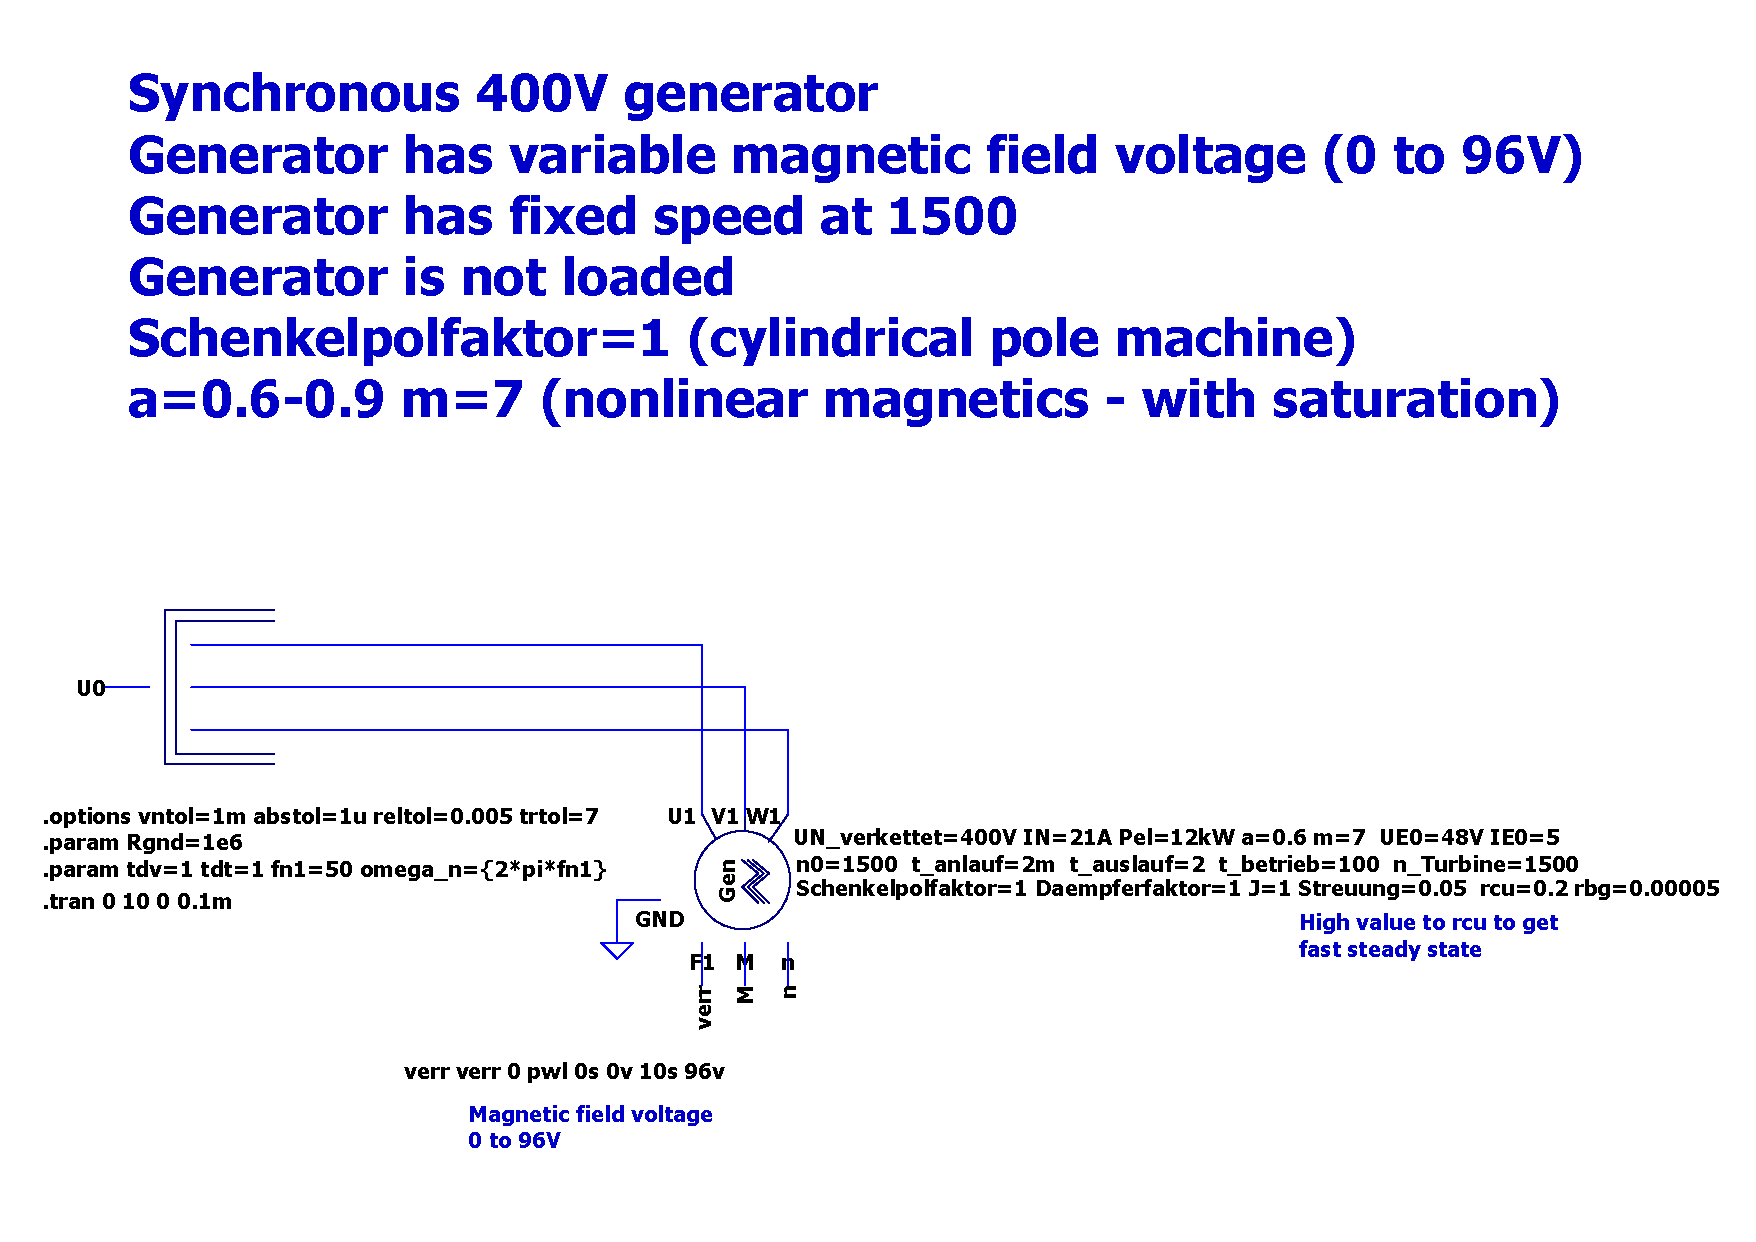
\includegraphics[width=1\textwidth] {figures/09_Synchronous_Generator_Characteristic_Curves_400V/sgen_400v_NoLoadLine_schematic.pdf}
	\caption{Open circuit characteristic - Schematic}
	\label{fig:figure91}
\end{figure}

\begin{figure}[H]
	\centering
	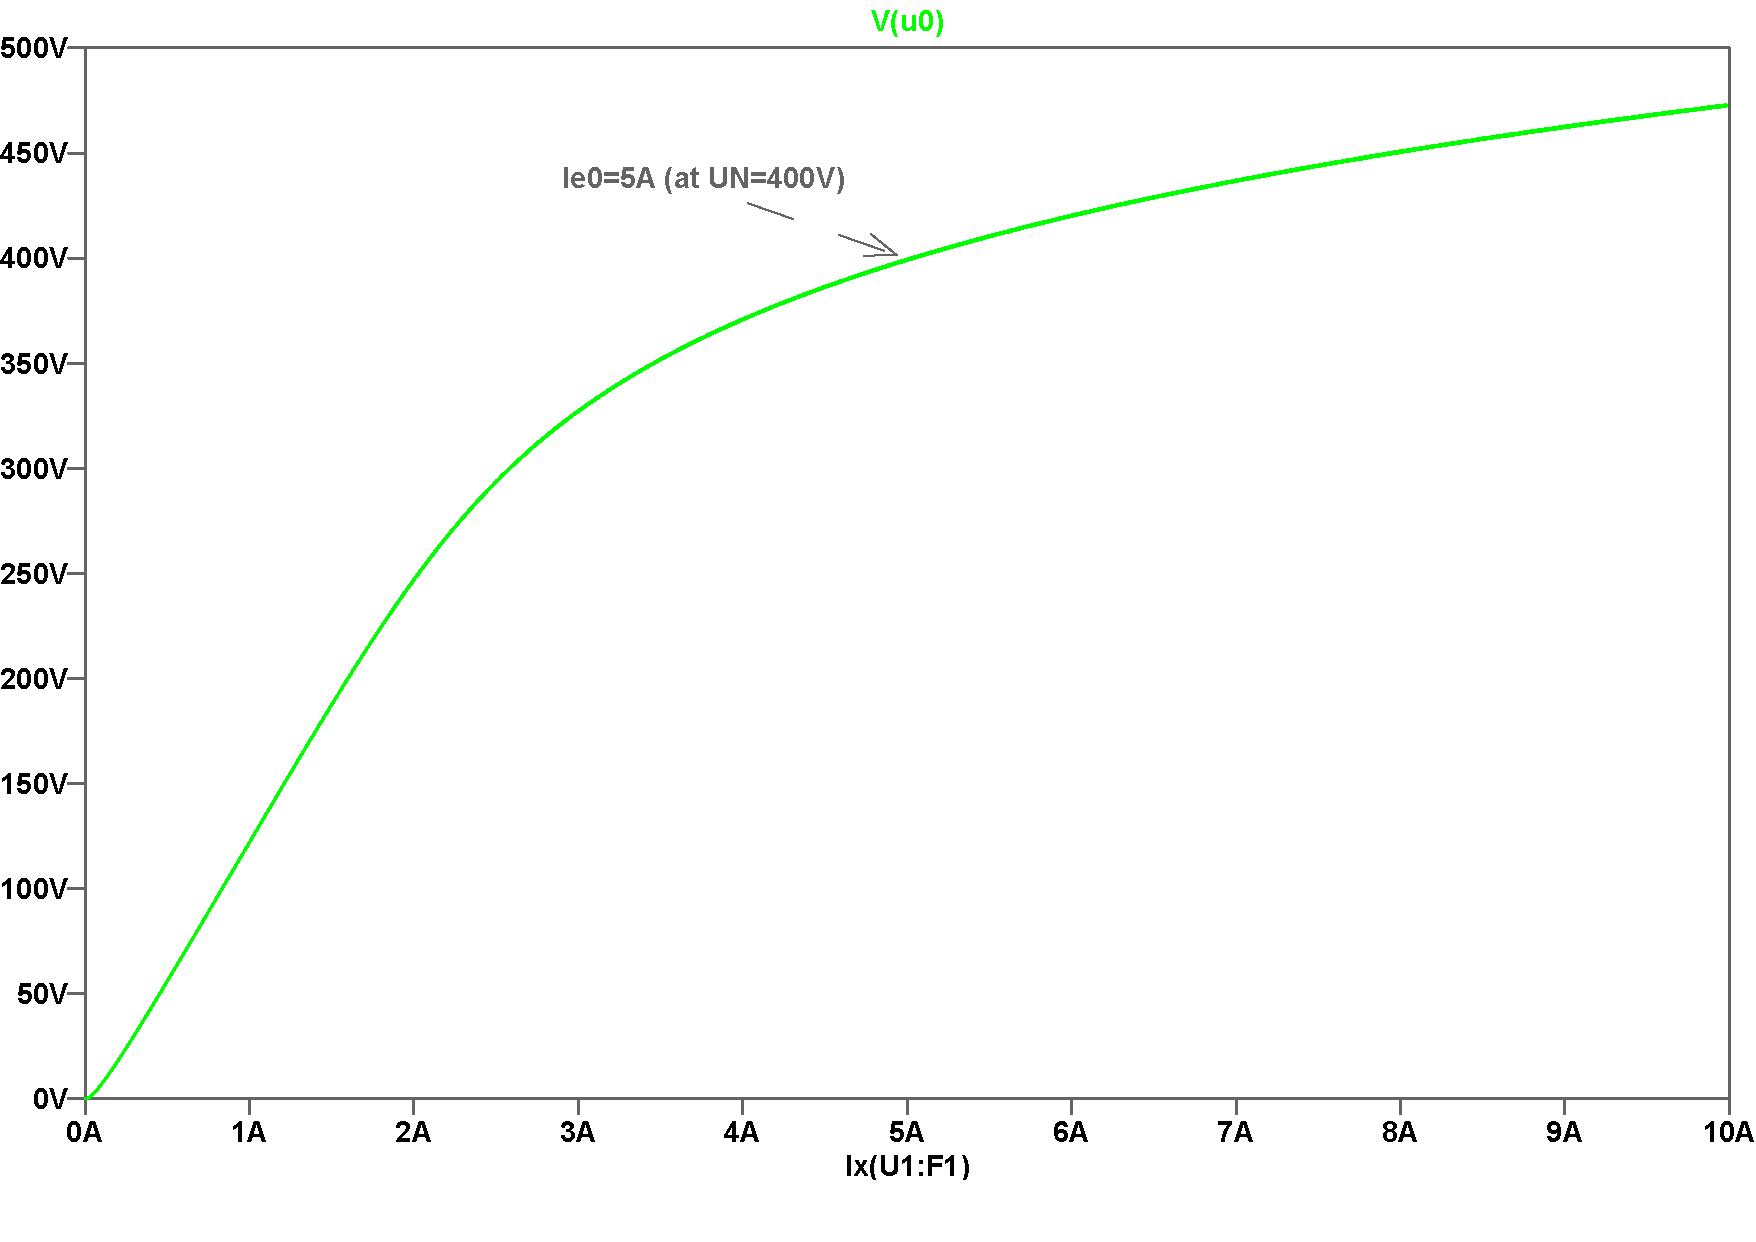
\includegraphics[width=0.9\textwidth] {figures/09_Synchronous_Generator_Characteristic_Curves_400V/sgen_400v_NoLoadLine_waveform.pdf}
	\caption{Open circuit characteristic - Waveform}
	\label{fig:figure92}
\end{figure}

\begin{itemize}
	\item determine the field current required for rated no-load voltage,
	\item investigate magnetic saturation and remanence,
	\item establish the air-gap line,
	\item estimate synchronous reactance and voltage regulation,
	\item determine the short-circuit ratio,
	\item select the operating range of the excitation system and AVR, and
	\item validate the saturation curve of a simulation model.
\end{itemize}

% ============================================================
\section{Short-Circuit Characteristic} see figure \ref{fig:figure93} and figure \ref{fig:figure94}  (simulation-file: same name as the heading) 
\label{sec:sg-scc}
% ============================================================

The short-circuit characteristic (SCC) describes the relationship between the
steady-state stator short-circuit current and the field current:

\begin{equation}
  I_k=f(I_f),
  \qquad U_s=0,
  \qquad n=n_N.
  \label{eq:sg-scc-definition}
\end{equation}

\subsection{Test Procedure}

The three stator terminals are short-circuited symmetrically through suitable
measuring equipment. The generator is driven at rated speed, and the
excitation is increased slowly from a small initial value. The corresponding
steady-state stator current is measured at each field-current setting.

\begin{important}{Current limitation during the test}{imp:sg-scc-safety}
The field current must be increased carefully. Rated stator current can be
reached at a field current considerably lower than that required for rated
open-circuit voltage. The conventional SCC test is normally stopped when the
rated stator current has been obtained.
\end{important}

\subsection{Shape of the Curve}

The short-circuit characteristic is approximately linear:

\begin{equation}
  I_k\propto I_f.
\end{equation}

During a symmetrical terminal short circuit, the terminal voltage is nearly
zero. The internal generated voltage is therefore balanced mainly by the
voltage drop across the synchronous impedance:

\begin{equation}
  \underline{E}
  \approx
  \left(R_s+\imag X_s\right)\underline{I}_k.
  \label{eq:sg-scc-phasor}
\end{equation}

Since normally $X_s\gg R_s$, the magnitude can be approximated by

\begin{equation}
  E\approx X_s I_k.
\end{equation}

The armature reaction is strongly demagnetizing during the symmetrical short
circuit. The resulting air-gap flux therefore remains comparatively small,
even when the stator current is high. The magnetic circuit operates mainly in
its unsaturated region, which explains the almost straight SCC.

\begin{figure}[H]
	\centering
	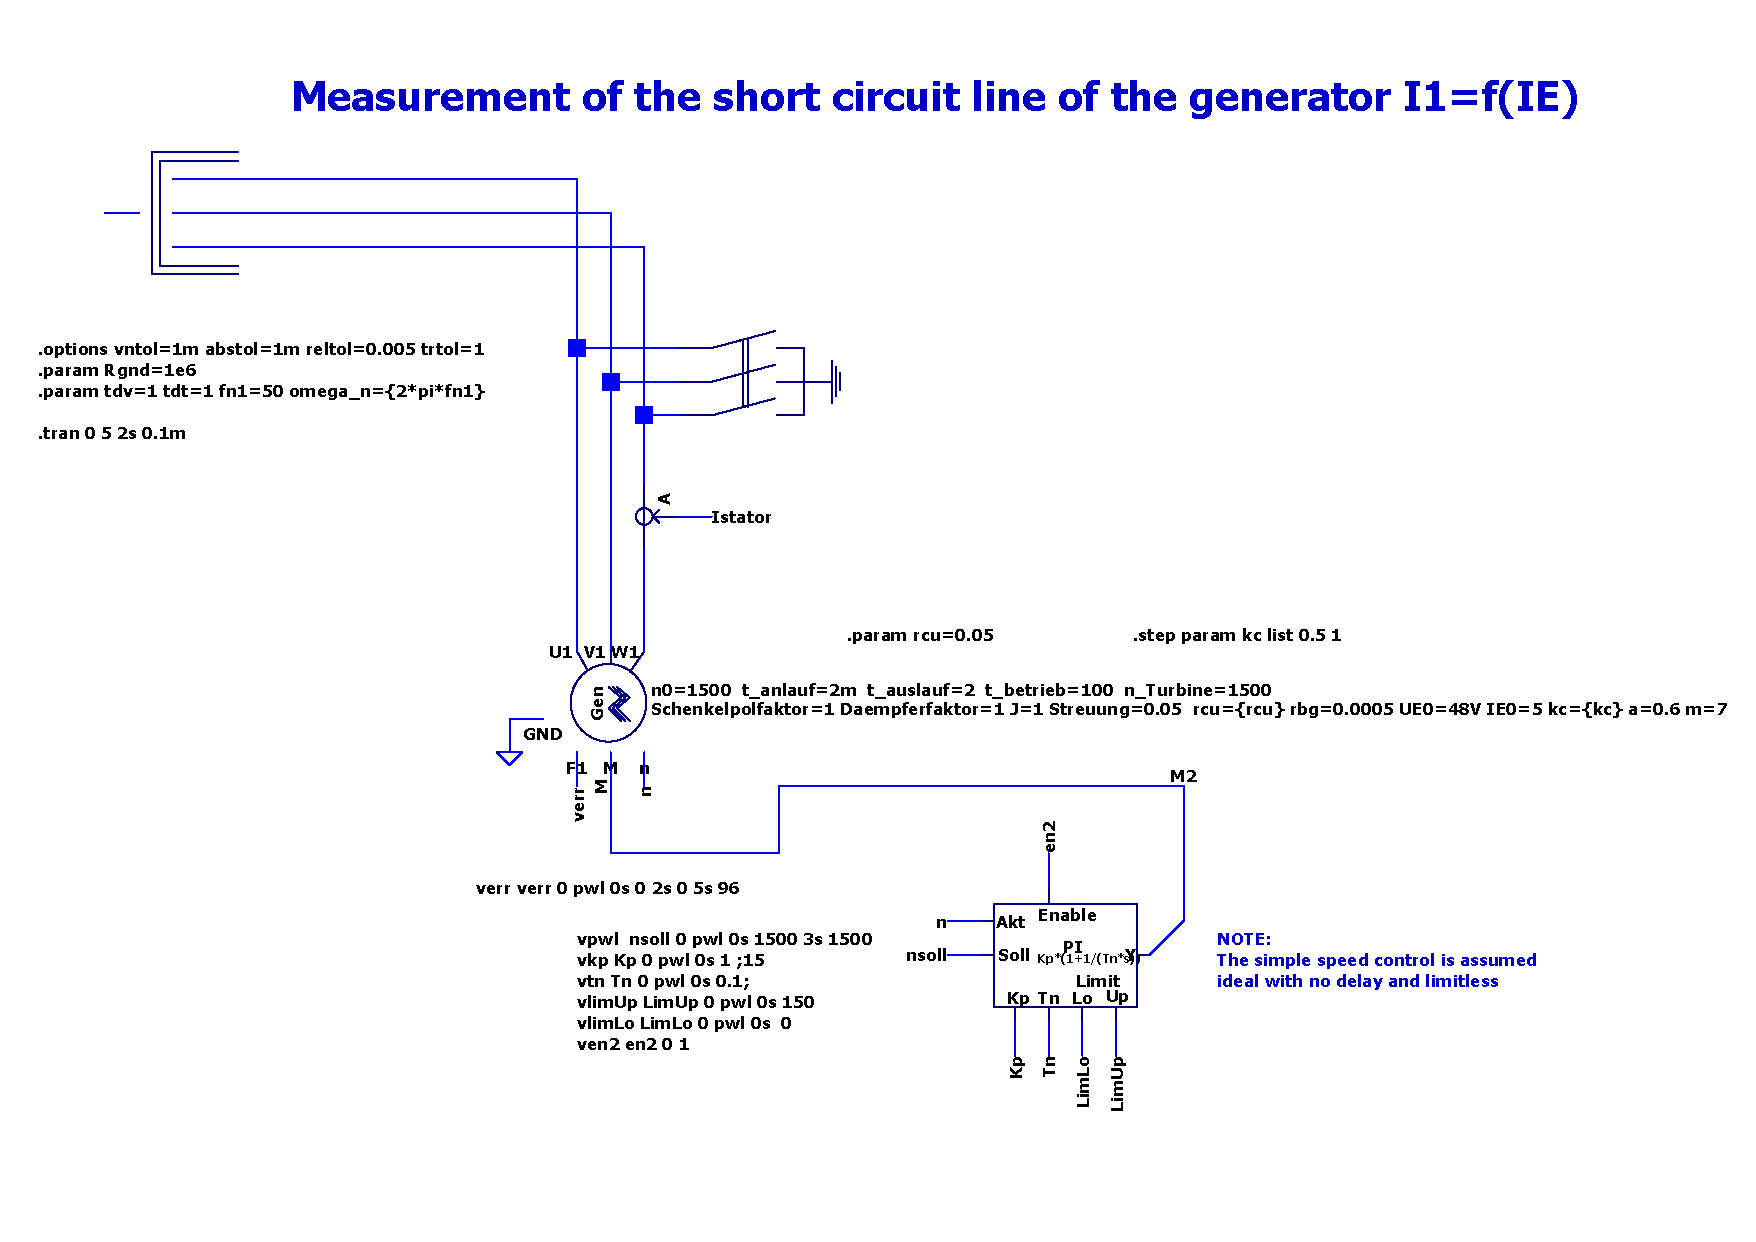
\includegraphics[width=0.9\textwidth] {figures/09_Synchronous_Generator_Characteristic_Curves_400V/sgen_400v_ShortCircuitLine_schematic.pdf}
	\caption{Short circuit characteristic - Schematic}
	\label{fig:figure93}
\end{figure}

\begin{figure}[H]
	\centering
	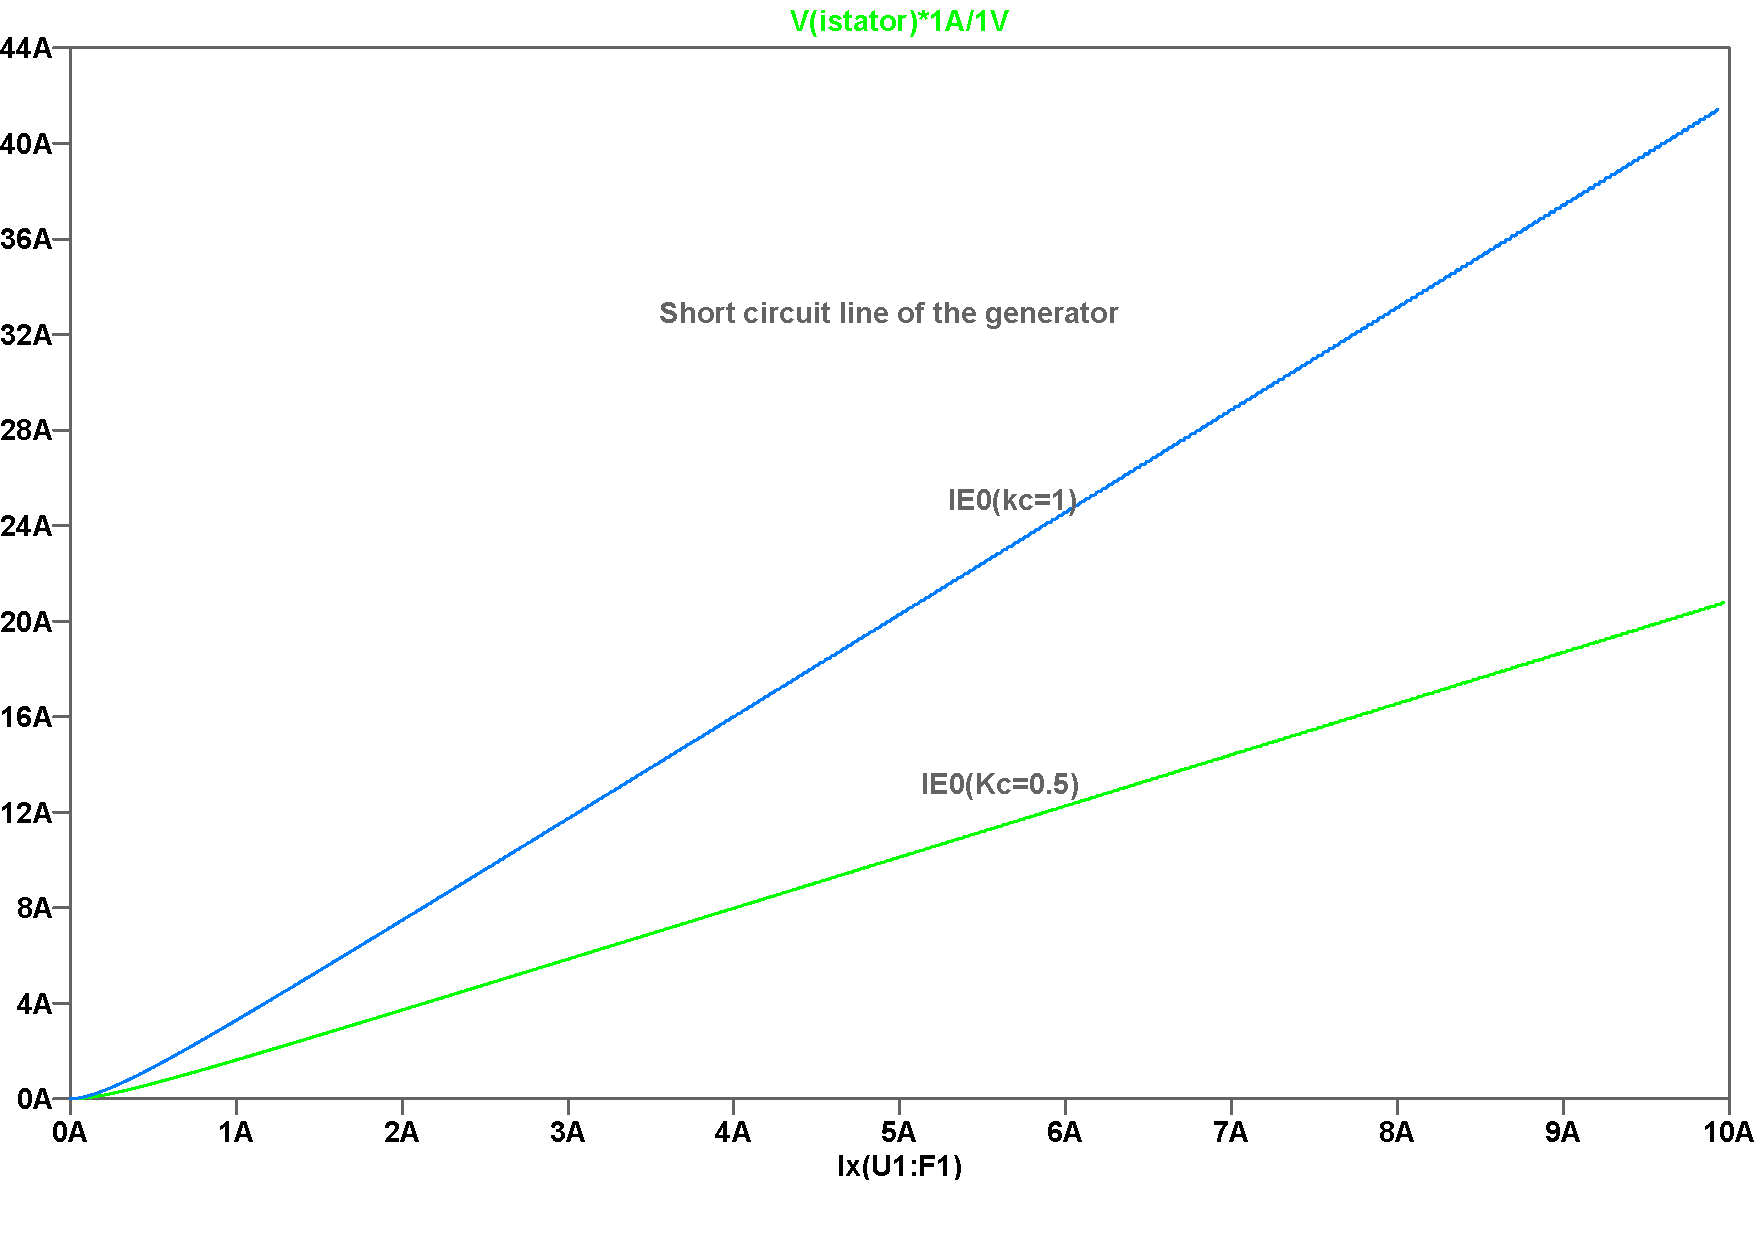
\includegraphics[width=0.9\textwidth] {figures/09_Synchronous_Generator_Characteristic_Curves_400V/sgen_400v_ShortCircuitLine_waveform.pdf}
	\caption{Short circuit characteristic - Waveform}
	\label{fig:figure94}
\end{figure}

The OCC is used to:


\subsection{Steady-State and Transient Short-Circuit Currents}

The conventional SCC represents the \emph{steady-state} short-circuit current.
Immediately after a sudden fault, however, the current is considerably higher
and passes through subtransient, transient, and steady-state intervals.

Neglecting resistance and using the appropriate direct-axis reactances, the
symmetrical AC components can be estimated as

\begin{align}
  I_k'' &\approx \frac{E}{X_d''},
  & \text{subtransient current}, \\
  I_k'  &\approx \frac{E}{X_d'},
  & \text{transient current}, \\
  I_k   &\approx \frac{E}{X_d},
  & \text{steady-state current}.
  \label{eq:sg-fault-current-stages}
\end{align}

The first interval is dominated by the stator and damper-winding flux
constraints. After the damper currents decay, the transient reactance becomes
effective. Finally, after the field transient has decayed, the current is
determined mainly by the synchronous reactance.

\begin{remark}{Sudden-fault waveform}{rem:sg-scc-transient}
The actual phase current following a sudden short circuit may also contain a
decaying DC component. Its magnitude depends on the fault inception angle and
the pre-fault operating point. The peak phase current can therefore be much
larger than the symmetrical RMS current represented by the SCC.
\end{remark}

\subsection{Synchronous-Impedance Estimate}

The OCC and SCC can be combined to estimate the synchronous impedance. The
open-circuit voltage and short-circuit current must be evaluated at the same
field current.

\begin{calculation}{Synchronous impedance from OCC and SCC}{calc:sg-zs-occ-scc}
Using phase voltage and phase current,
\begin{align}
  Z_s &= \frac{U_{0,\mathrm{ph}}}{I_k}, \\
  X_s &= \sqrt{Z_s^2-R_s^2}.
\end{align}

If the stator resistance is small compared with the reactance,
\begin{equation}
  X_s\approx Z_s.
\end{equation}
\end{calculation}

The OCC may already be saturated at the selected field current, whereas the
SCC remains almost unsaturated. The synchronous-impedance method therefore
usually gives a conservative, relatively high estimate of voltage regulation.

\subsection{Short-Circuit Ratio}

The short-circuit ratio is commonly defined as

\begin{equation}
  \mathrm{SCR}
  =\frac{I_{f,U_N}}{I_{f,I_N}},
  \label{eq:sg-scr}
\end{equation}

where $I_{f,U_N}$ is the field current required to produce rated voltage on
open circuit and $I_{f,I_N}$ is the field current required to produce rated
stator current under steady-state short-circuit conditions. Approximately,

\begin{equation}
  \mathrm{SCR}\approx\frac{1}{x_d},
\end{equation}

when $x_d$ is expressed in per unit. Saturation and the exact test definition
affect this relationship.

A comparatively large SCR generally indicates a smaller synchronous
reactance, improved steady-state voltage regulation, and a larger stability
margin. It also leads to higher short-circuit current and usually requires a
physically larger and more expensive machine.

\newpage

% ============================================================
\section{Load or External Characteristic} see figure \ref{fig:figure95}-\ref{fig:figure910}  (simulation-files: same names as the headings) 
\label{sec:sg-load-characteristic}
% ============================================================

The load characteristic describes how the generator terminal voltage changes
with stator current when speed, field current, and load power factor remain
constant:

\begin{equation}
  U=f(I_s),
  \qquad
  n=\text{constant},
  \qquad
  I_f=\text{constant},
  \qquad
  \cos\varphi=\text{constant}.
  \label{eq:sg-load-characteristic}
\end{equation}

It is therefore also called the \emph{external characteristic} of the
generator.

For a simplified round-rotor generator, the steady-state phasor equation is

\begin{equation}
  \underline{E}
  =\underline{U}
  +\left(R_s+\imag X_s\right)\underline{I}_s.
  \label{eq:sg-generator-phasor}
\end{equation}

If field current and speed are constant, the magnitude of $E$ is approximately
constant. The terminal voltage must consequently change when the stator current
changes. The direction and magnitude of this voltage change depend strongly on
the load power factor.

\subsection{Inductive Load}

For a lagging load, the stator current lags behind the terminal voltage. The
reactive voltage drop $\imag X_s\underline{I}_s$ and the demagnetizing armature
reaction reduce the terminal voltage. Consequently, the voltage falls
significantly as the load current rises, and the external characteristic has a
pronounced negative slope.

\subsection{Unity-Power-Factor Load}

At unity power factor, stator current and terminal voltage are in phase. The
terminal voltage still decreases as the current increases, but usually less
strongly than for an inductive load. The reduction results from stator
resistance, synchronous reactance, armature reaction, and magnetic saturation.

\subsection{Capacitive Load}

For a leading load, the stator current leads the terminal voltage. The armature
reaction can then have a magnetizing effect. As the current increases, the
terminal voltage may remain nearly constant or even rise. The external
characteristic can therefore have a positive slope.

This behaviour explains why capacitive loads and overexcited synchronous
machines can support the voltage of a power system.


\subsection{Voltage Regulation}

The voltage regulation of a synchronous generator is commonly expressed as

\begin{equation}
  \varepsilon_U
  =\frac{U_0-U_N}{U_N}\cdot100\%,
  \label{eq:sg-voltage-regulation}
\end{equation}

where $U_0$ is the no-load voltage obtained after removing the load without
changing speed or field current, and $U_N$ is the terminal voltage at the
specified load.

For an inductive load, the regulation is normally positive because
$U_0>U_N$. For a sufficiently capacitive load, it may become negative because
the loaded terminal voltage can exceed the corresponding no-load voltage.

% ============================================================

\begin{figure}[H]
	\centering
	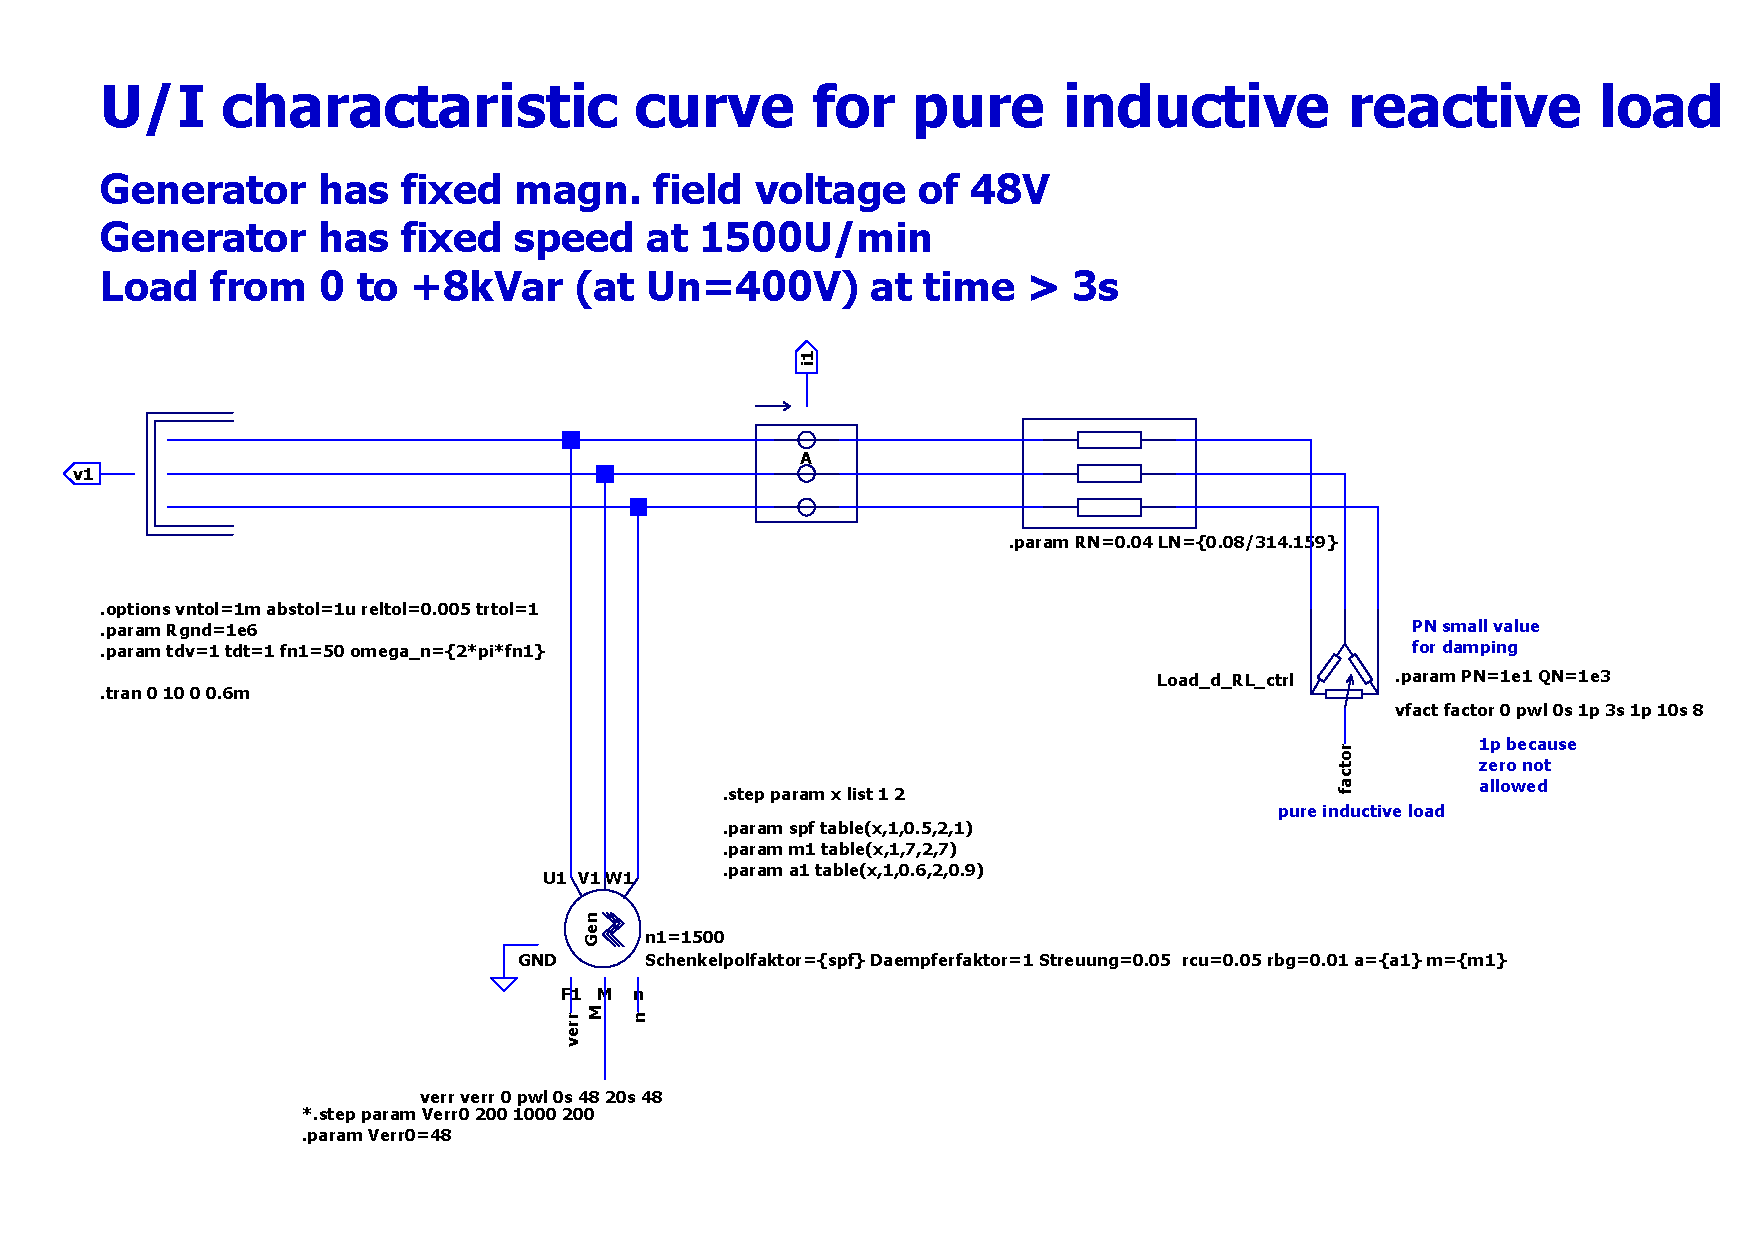
\includegraphics[width=0.9\textwidth] {figures/09_Synchronous_Generator_Characteristic_Curves_400V/sgen_400v_constant_speed_loadcurve_induktiv_schematic.pdf}
	\caption{Inductive characteristic - Schematic}
	\label{fig:figure95}
\end{figure}

\begin{figure}[H]
	\centering
	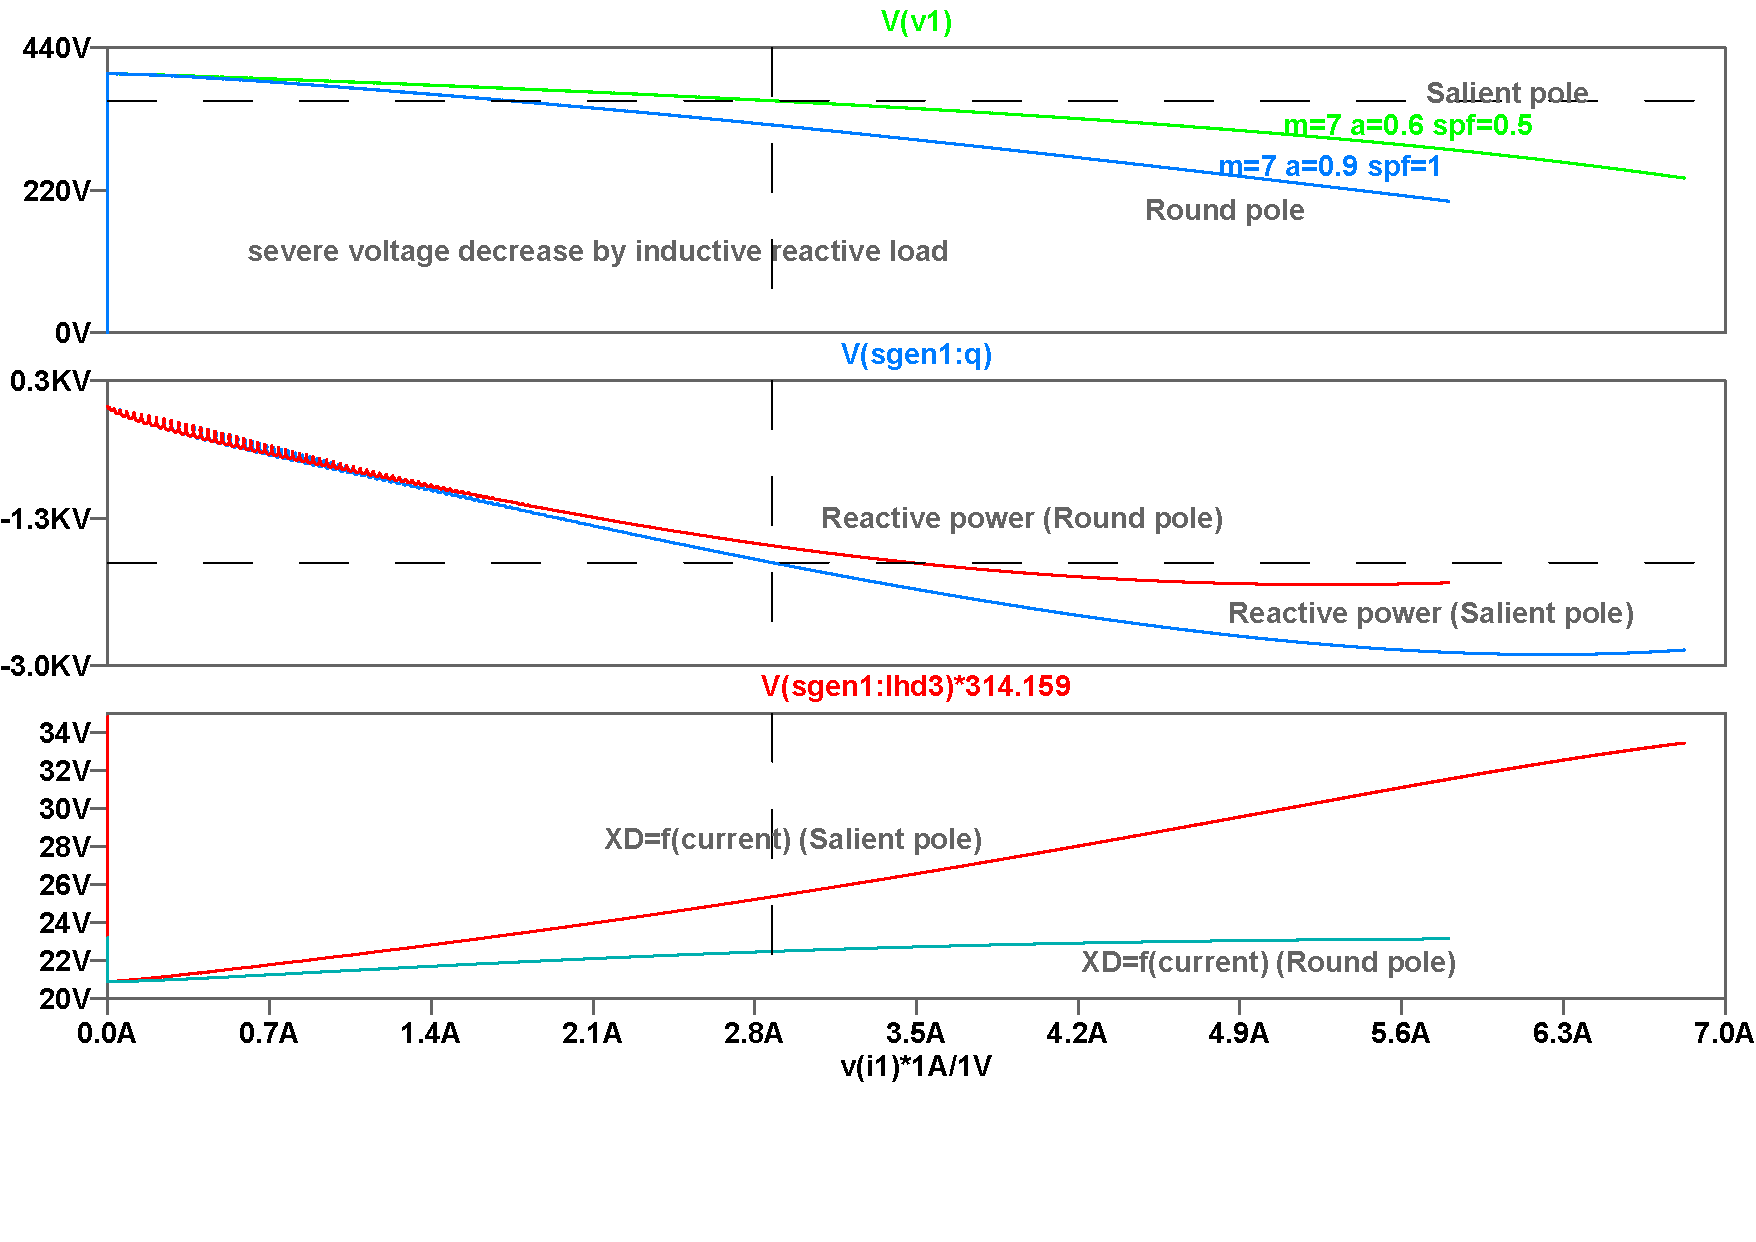
\includegraphics[width=0.9\textwidth] {figures/09_Synchronous_Generator_Characteristic_Curves_400V/sgen_400v_constant_speed_loadcurve_induktiv_waveform.pdf}
	\caption{Inductive characteristic - Waveform}
	\label{fig:figure96}
\end{figure}

\begin{figure}[H]
	\centering
	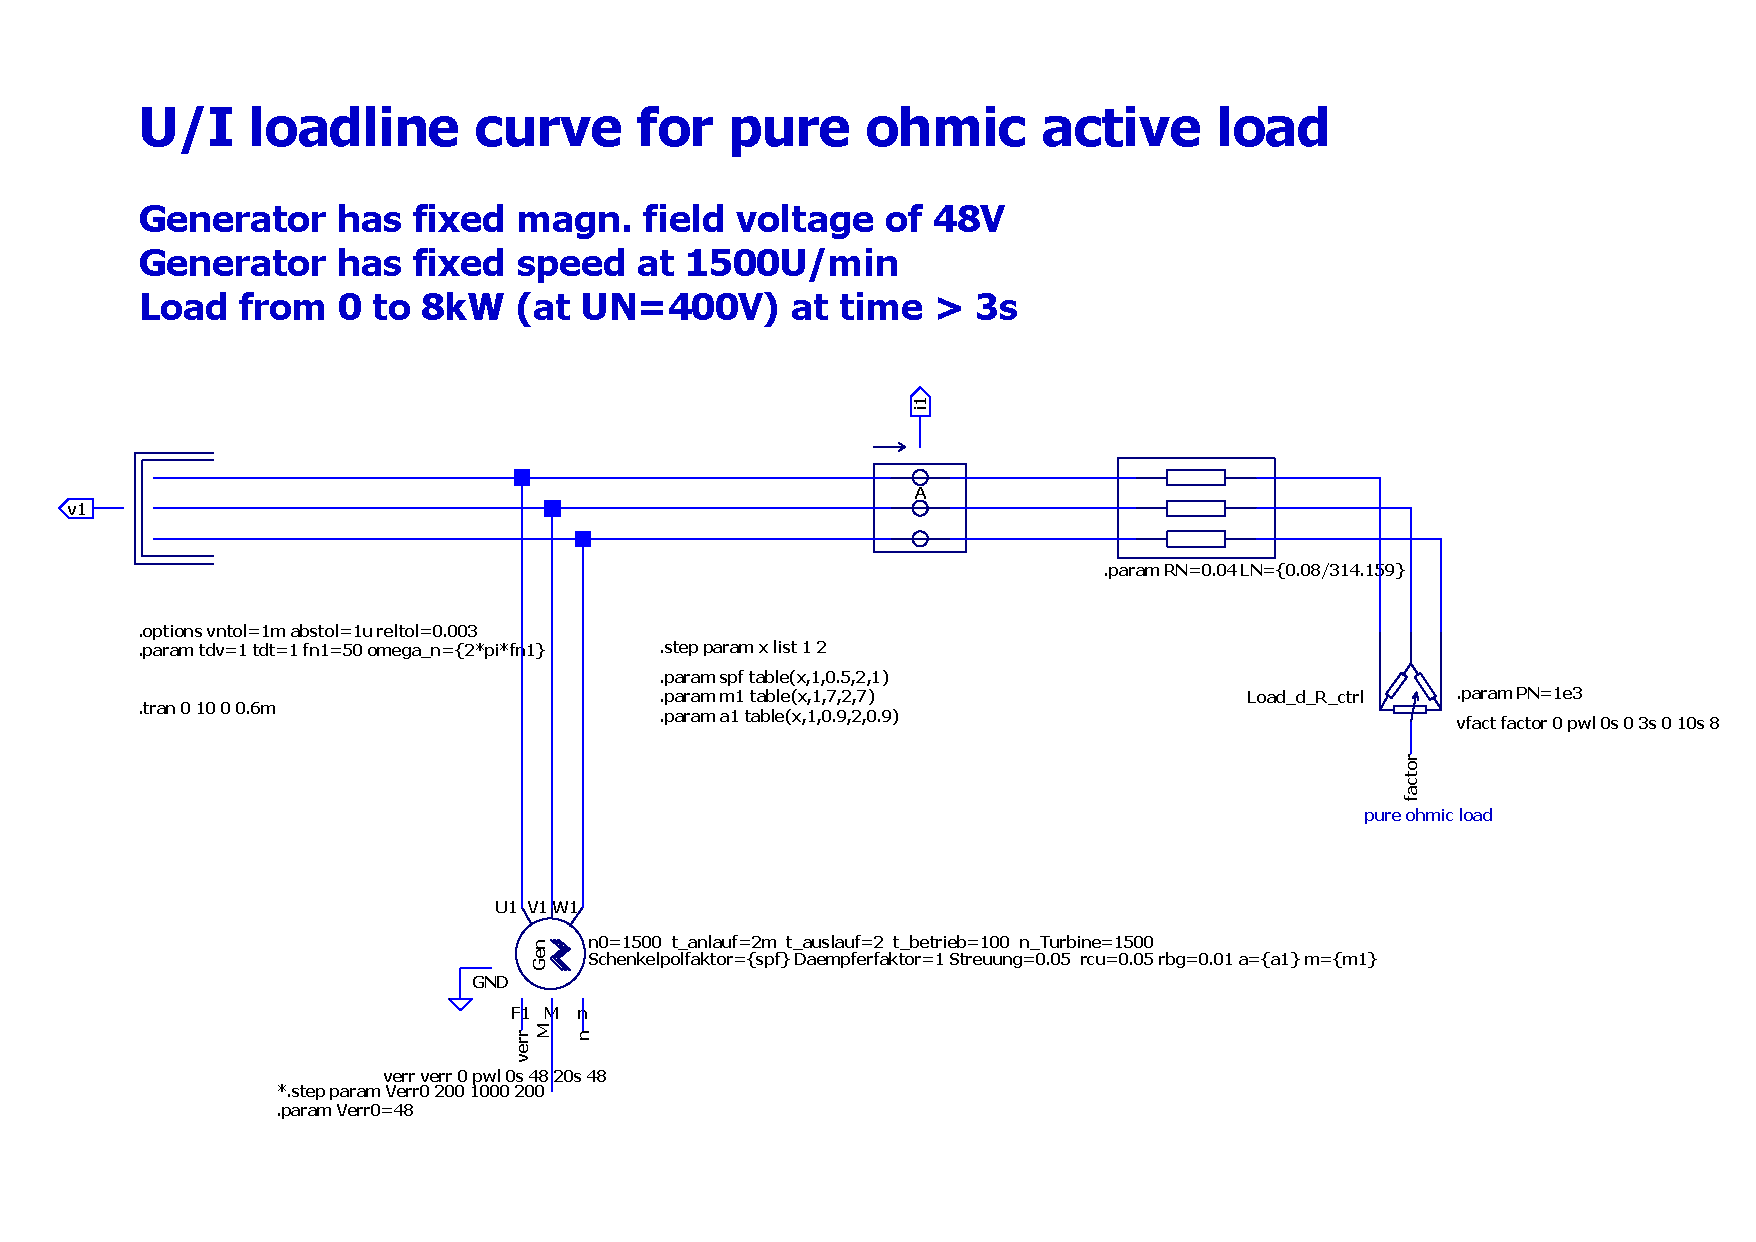
\includegraphics[width=0.9\textwidth] {figures/09_Synchronous_Generator_Characteristic_Curves_400V/sgen_400v_constant_speed_loadcurve_ohmic_schematic.pdf}
	\caption{Resistive characteristic - Schematic}
	\label{fig:figure97}
\end{figure}

\begin{figure}[H]
	\centering
	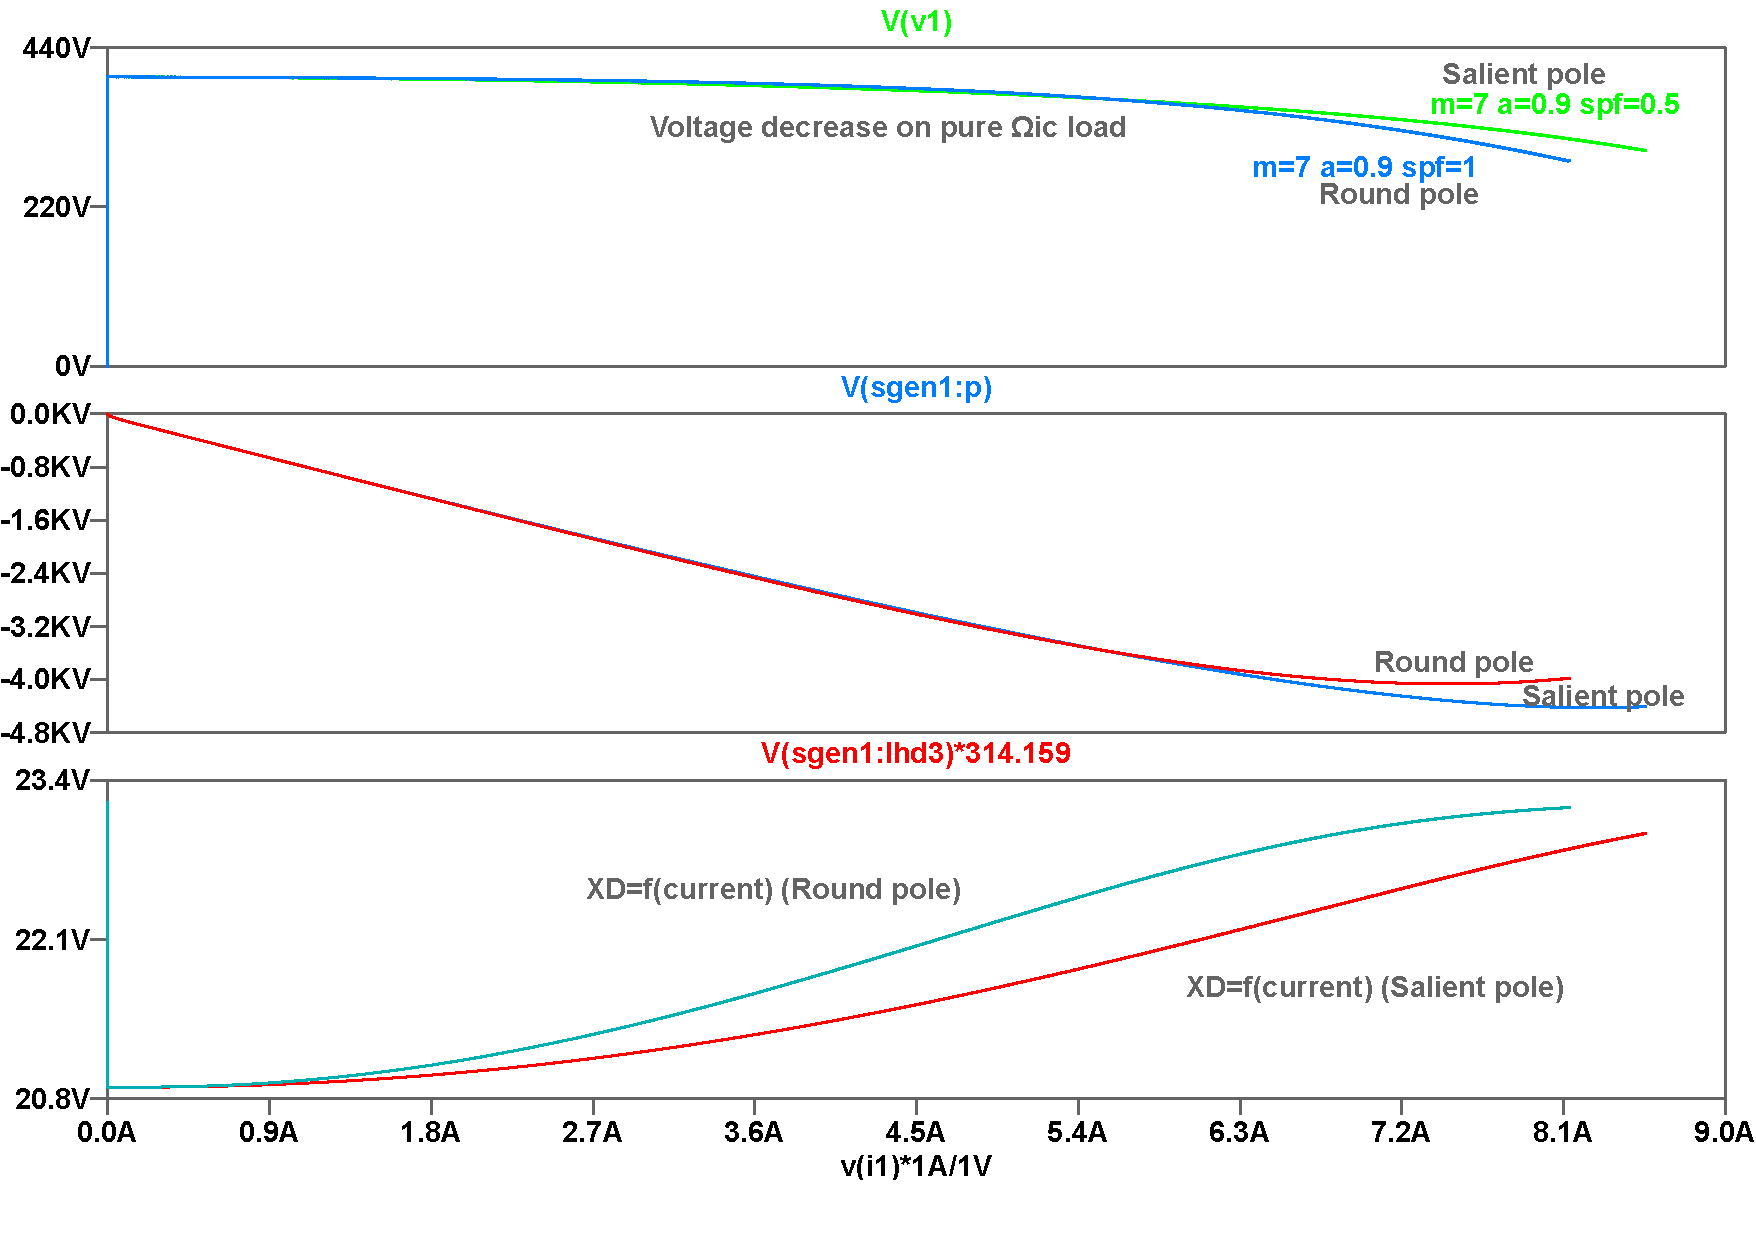
\includegraphics[width=0.9\textwidth] {figures/09_Synchronous_Generator_Characteristic_Curves_400V/sgen_400v_constant_speed_loadcurve_ohmic_waveform.pdf}
	\caption{Resistive characteristic - Waveform}
	\label{fig:figure98}
\end{figure}

\begin{figure}[H]
	\centering
	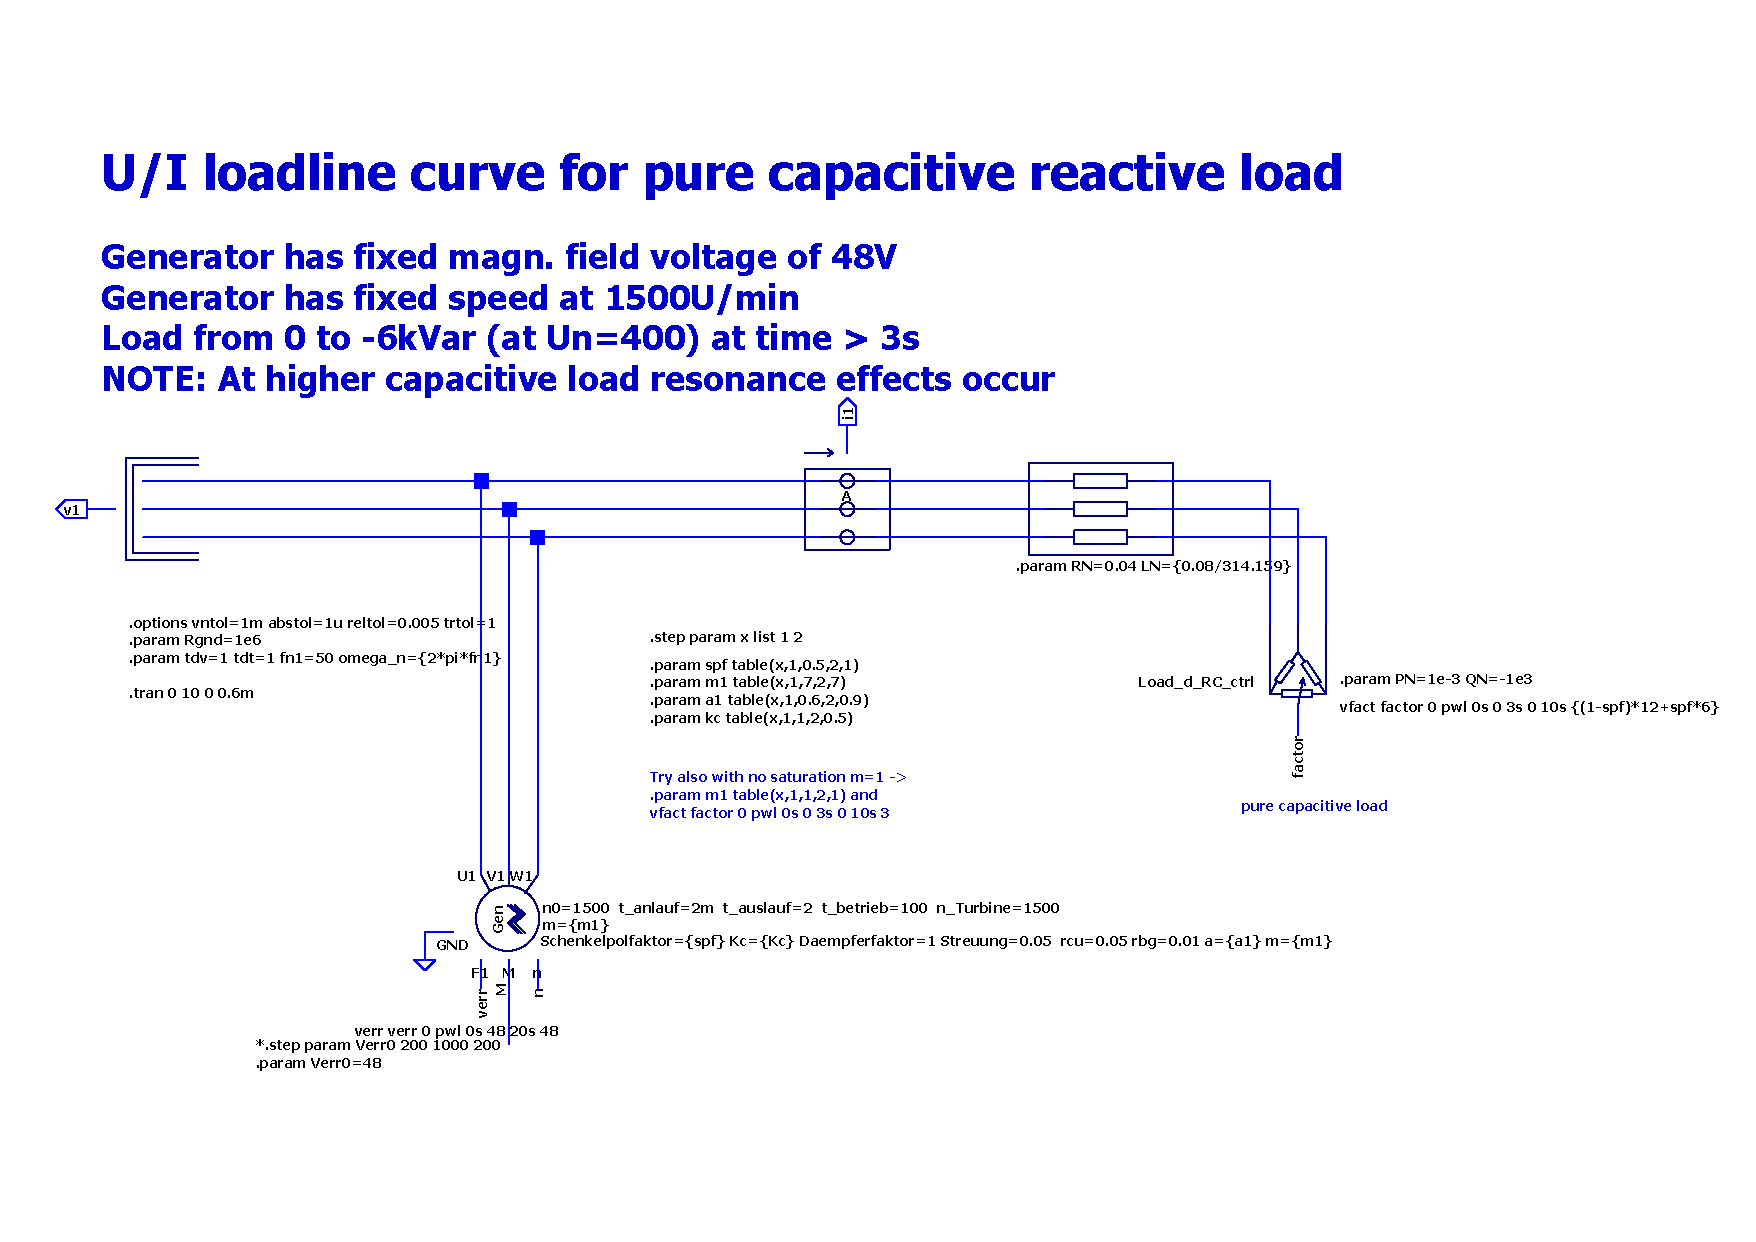
\includegraphics[width=0.9\textwidth] {figures/09_Synchronous_Generator_Characteristic_Curves_400V/sgen_400v_constant_speed_loadcurve_capacitive_schematic.pdf}
	\caption{Capacitive characteristic - Schematic}
	\label{fig:figure99}
\end{figure}

\begin{figure}[H]
	\centering
	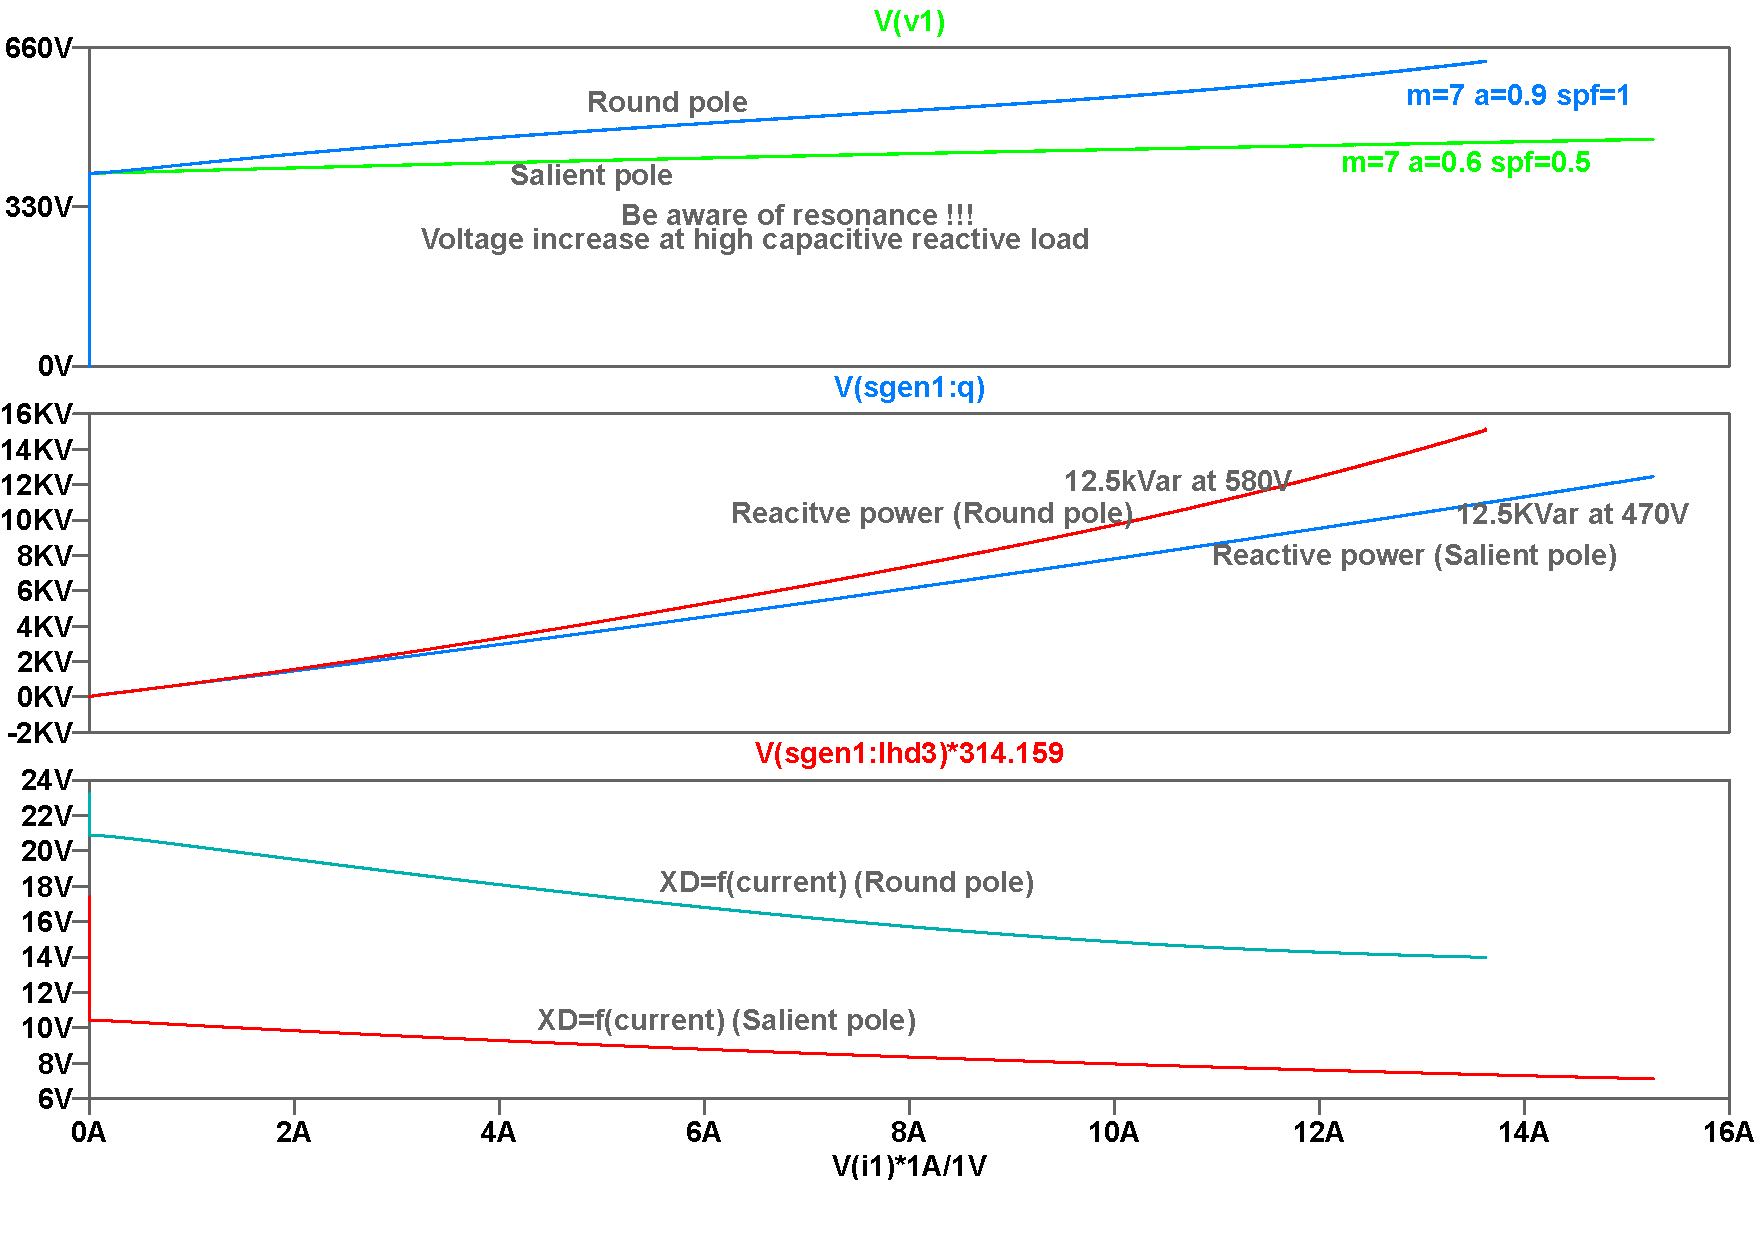
\includegraphics[width=0.9\textwidth] {figures/09_Synchronous_Generator_Characteristic_Curves_400V/sgen_400v_constant_speed_loadcurve_capacitive_waveform.pdf}
	\caption{Capacitive characteristic - Waveform}
	\label{fig:figure910}
\end{figure}

\section{Regulation Characteristic} see figures \ref{fig:figure911}-\ref{fig:figure916}  (simulation-file: same names as the headings) 
\label{sec:sg-regulation-characteristic}
% ============================================================

The regulation characteristic describes the field current required to
maintain constant terminal voltage while the stator current changes:

\begin{equation}
  I_f=f(I_s),
  \qquad
  U=U_N,
  \qquad
  n=n_N,
  \qquad
  \cos\varphi=\text{constant}.
  \label{eq:sg-regulation-characteristic}
\end{equation}

It is sometimes called the excitation characteristic under load.

\begin{important}{Difference between load and regulation characteristics}
  {imp:sg-load-versus-regulation}
The load characteristic gives $U=f(I_s)$ at constant excitation. The
regulation characteristic gives $I_f=f(I_s)$ while the terminal voltage is
kept constant. The two characteristics therefore describe complementary
operating conditions.
\end{important}

\subsection{Inductive Load}

For a lagging load, armature reaction is predominantly demagnetizing, and the
synchronous-reactance voltage drop increases with stator current. The
excitation must therefore be increased as the load rises:

\begin{equation}
  I_s\uparrow
  \quad\Longrightarrow\quad
  I_f\uparrow.
\end{equation}

The regulation curve consequently rises relatively steeply.

\subsection{Unity-Power-Factor Load}

At unity power factor, the required field current normally increases with
stator current, but less strongly than for an inductive load.

\subsection{Capacitive Load}

For a leading load, armature reaction is partly magnetizing. Less field current
is therefore required to maintain rated terminal voltage. Over part of the
operating range,

\begin{equation}
  I_s\uparrow
  \quad\Longrightarrow\quad
  I_f\downarrow.
\end{equation}

For strongly capacitive operating conditions, the generator may therefore
have to operate underexcited.

\subsection{Practical Importance}

The regulation characteristic is directly related to the task of the AVR.
When load current and power factor change, the AVR adjusts field voltage and
field current so that the terminal voltage remains at its reference value.

%The characteristic is useful for:
%
%\begin{itemize}
%  \item selecting the required excitation-voltage and field-current range,
%  \item designing and limiting the AVR,
%  \item estimating reactive-power requirements,
%  \item checking rotor field-winding heating, and
%  \item determining permissible underexcited operation.
%\end{itemize}

%\begin{remark}{Static and dynamic regulation}{rem:sg-static-regulation}
%The regulation characteristic contains steady-state operating points. It does
%not describe the transient response, stability, or time constants of the AVR
%and excitation system.
%\end{remark}

\begin{figure}[H]
	\centering
	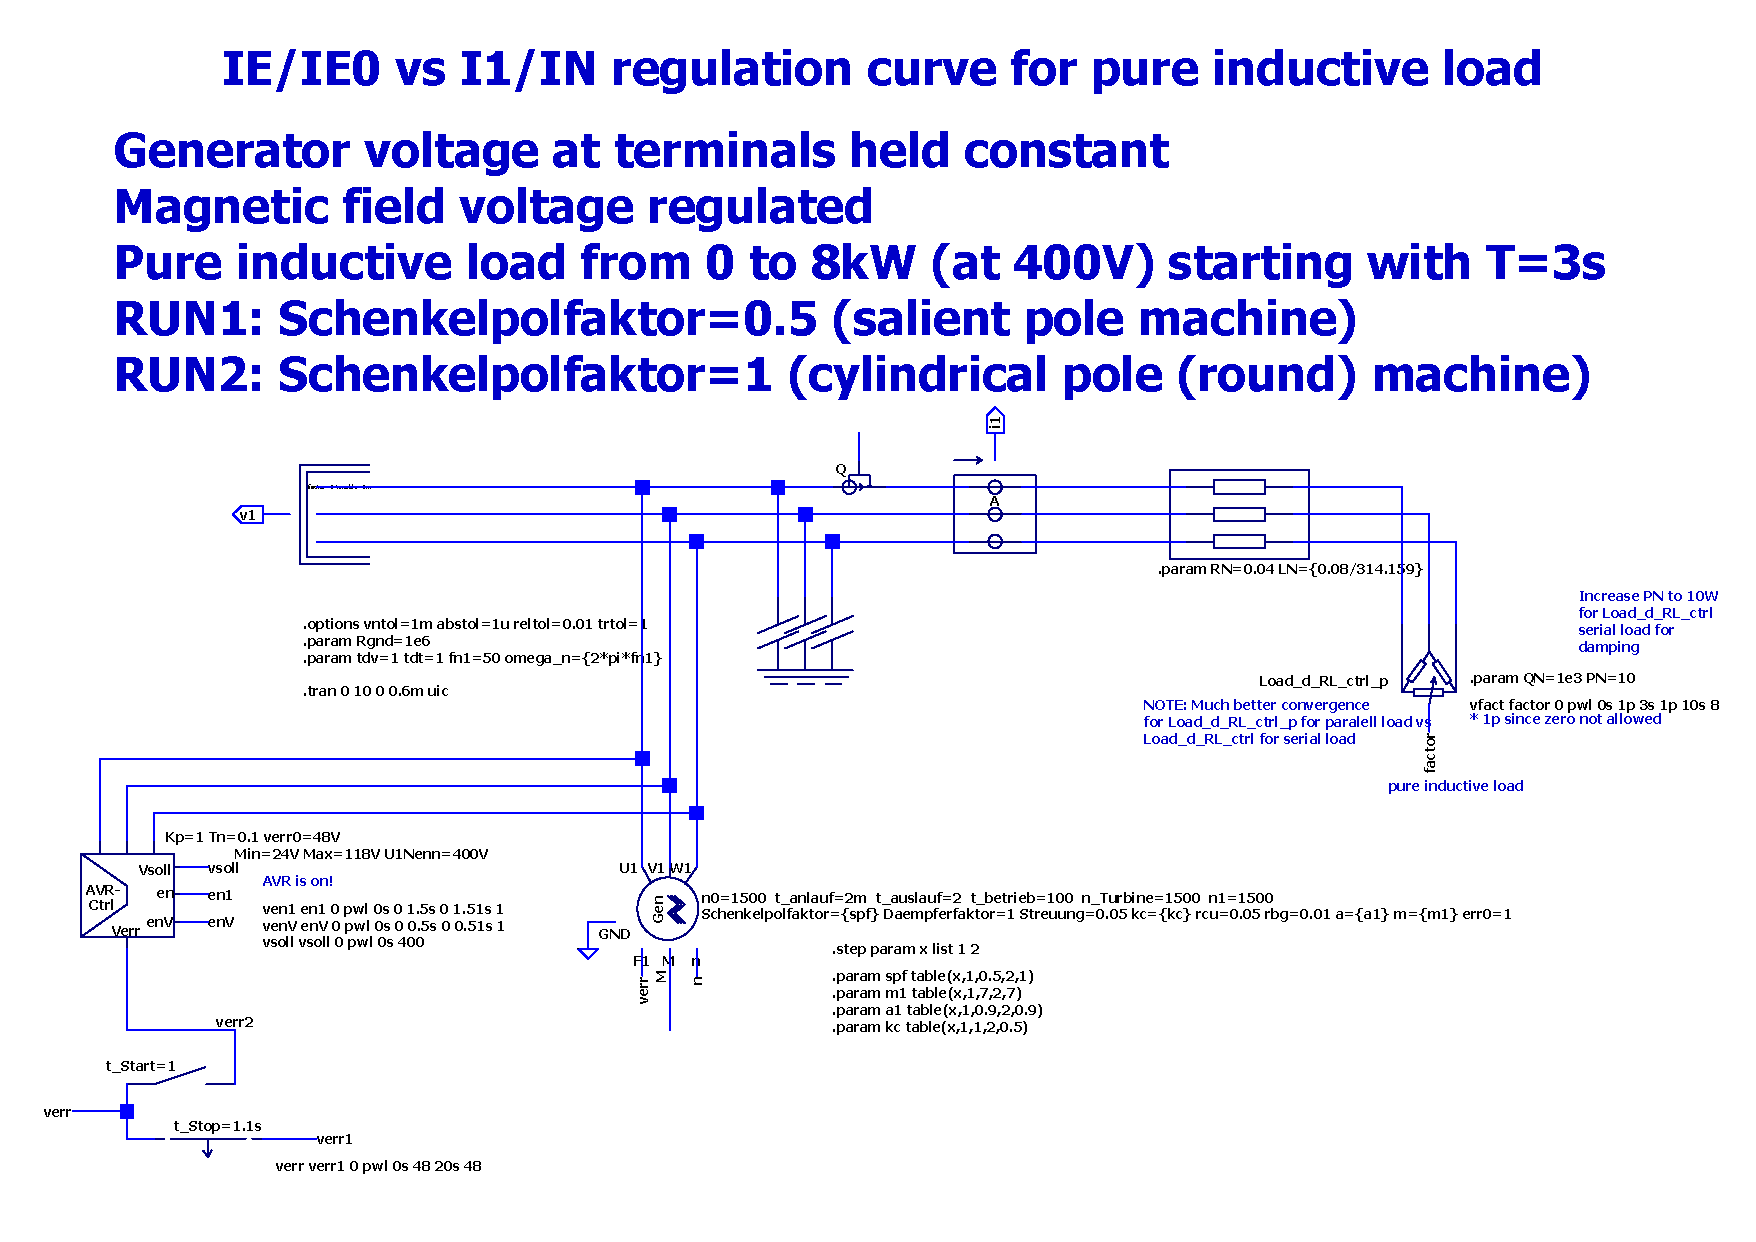
\includegraphics[width=0.9\textwidth] {figures/09_Synchronous_Generator_Characteristic_Curves_400V/sgen_400V_Regulationcurve_inductive_schematic.pdf}
	\caption{Inductive Regulation curve - Schematic}
	\label{fig:figure911}
\end{figure}

\begin{figure}[H]
	\centering
	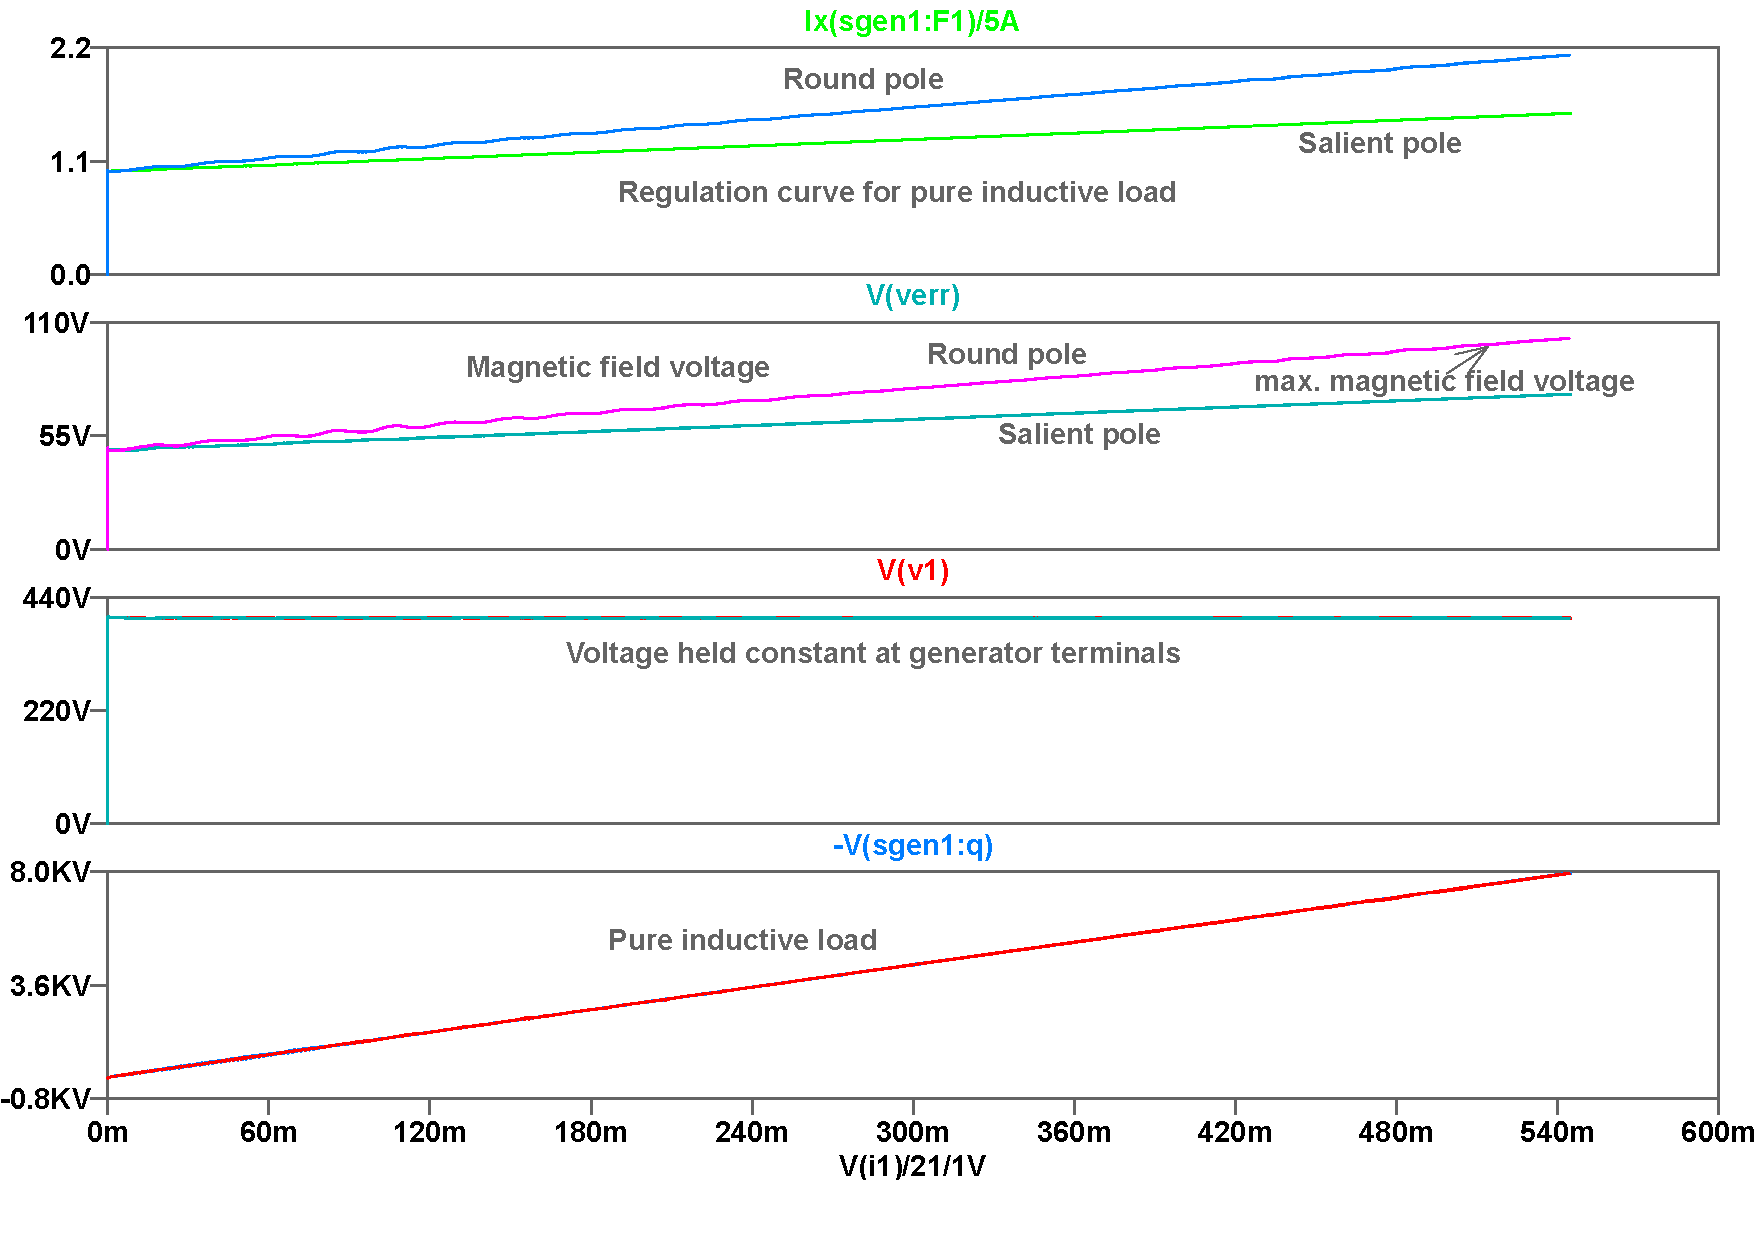
\includegraphics[width=0.9\textwidth] {figures/09_Synchronous_Generator_Characteristic_Curves_400V/sgen_400V_Regulationcurve_inductive_waveform.pdf}
	\caption{Inductive Regulation curve - Waveform}
	\label{fig:figure912}
\end{figure}

\begin{figure}[H]
	\centering
	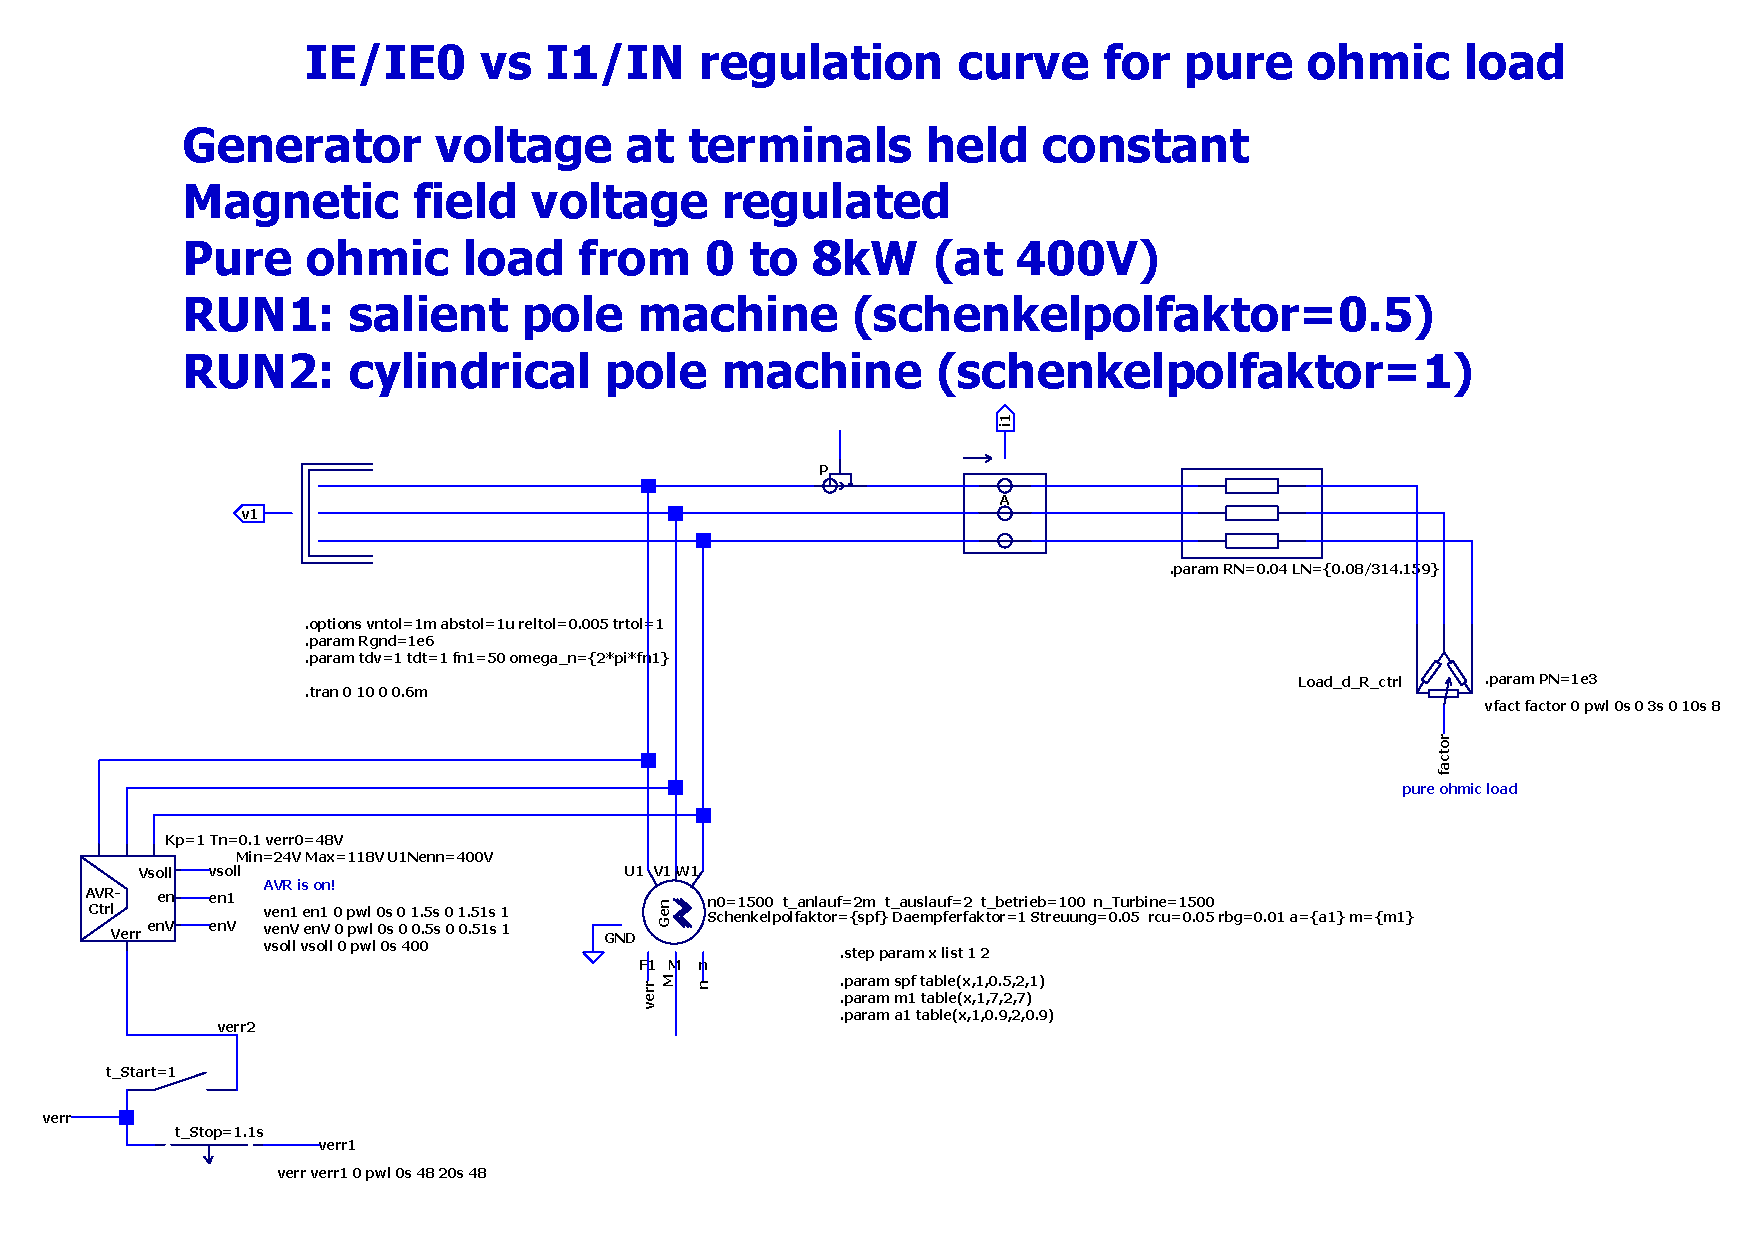
\includegraphics[width=0.9\textwidth] {figures/09_Synchronous_Generator_Characteristic_Curves_400V/sgen_400V_Regulationcurve_ohmic_schematic.pdf}
	\caption{Ohmic  Regulation curve - Schematic}
	\label{fig:figure913}
\end{figure}

\begin{figure}[H]
	\centering
	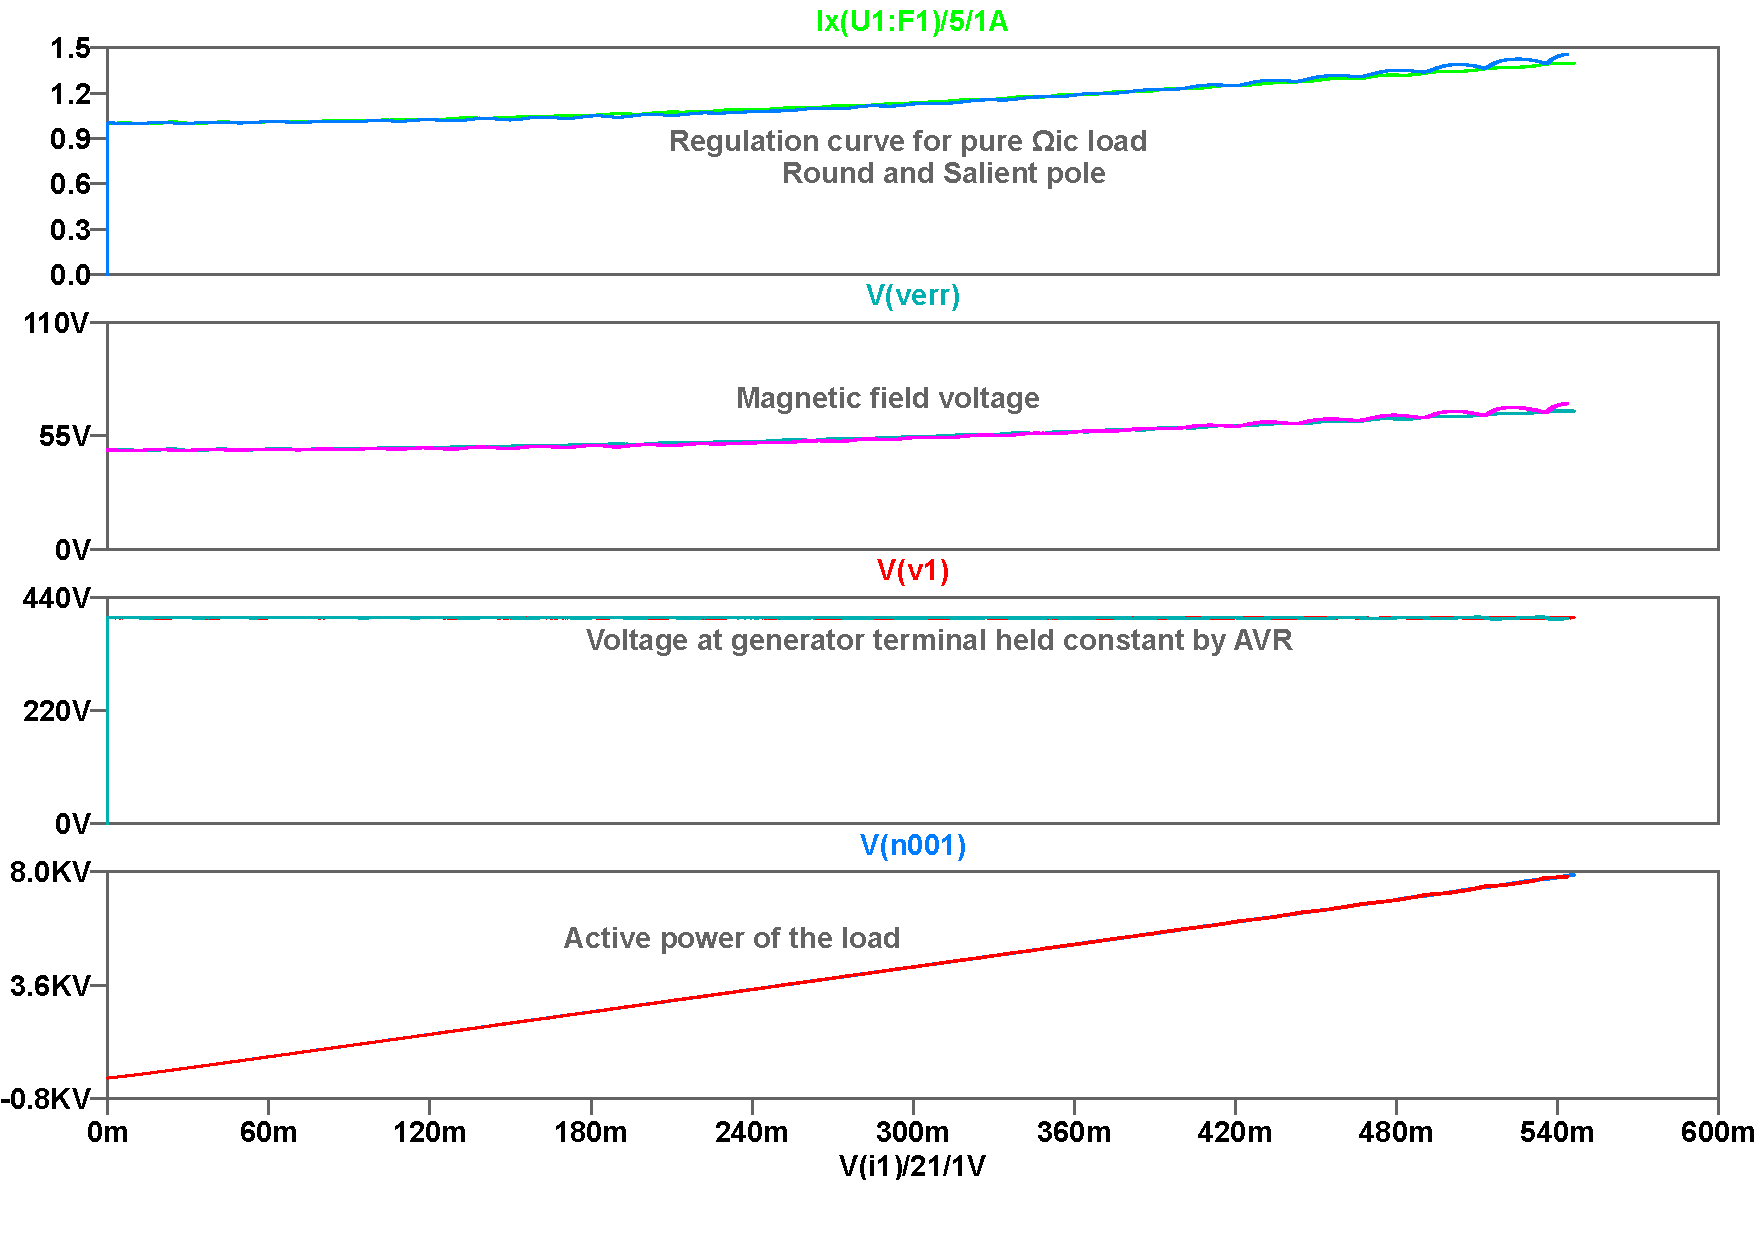
\includegraphics[width=0.9\textwidth] {figures/09_Synchronous_Generator_Characteristic_Curves_400V/sgen_400V_Regulationcurve_ohmic_waveform.pdf}
	\caption{Ohmic  Regulation curve - Waveform}
	\label{fig:figure914}
\end{figure}

\begin{figure}[H]
	\centering
	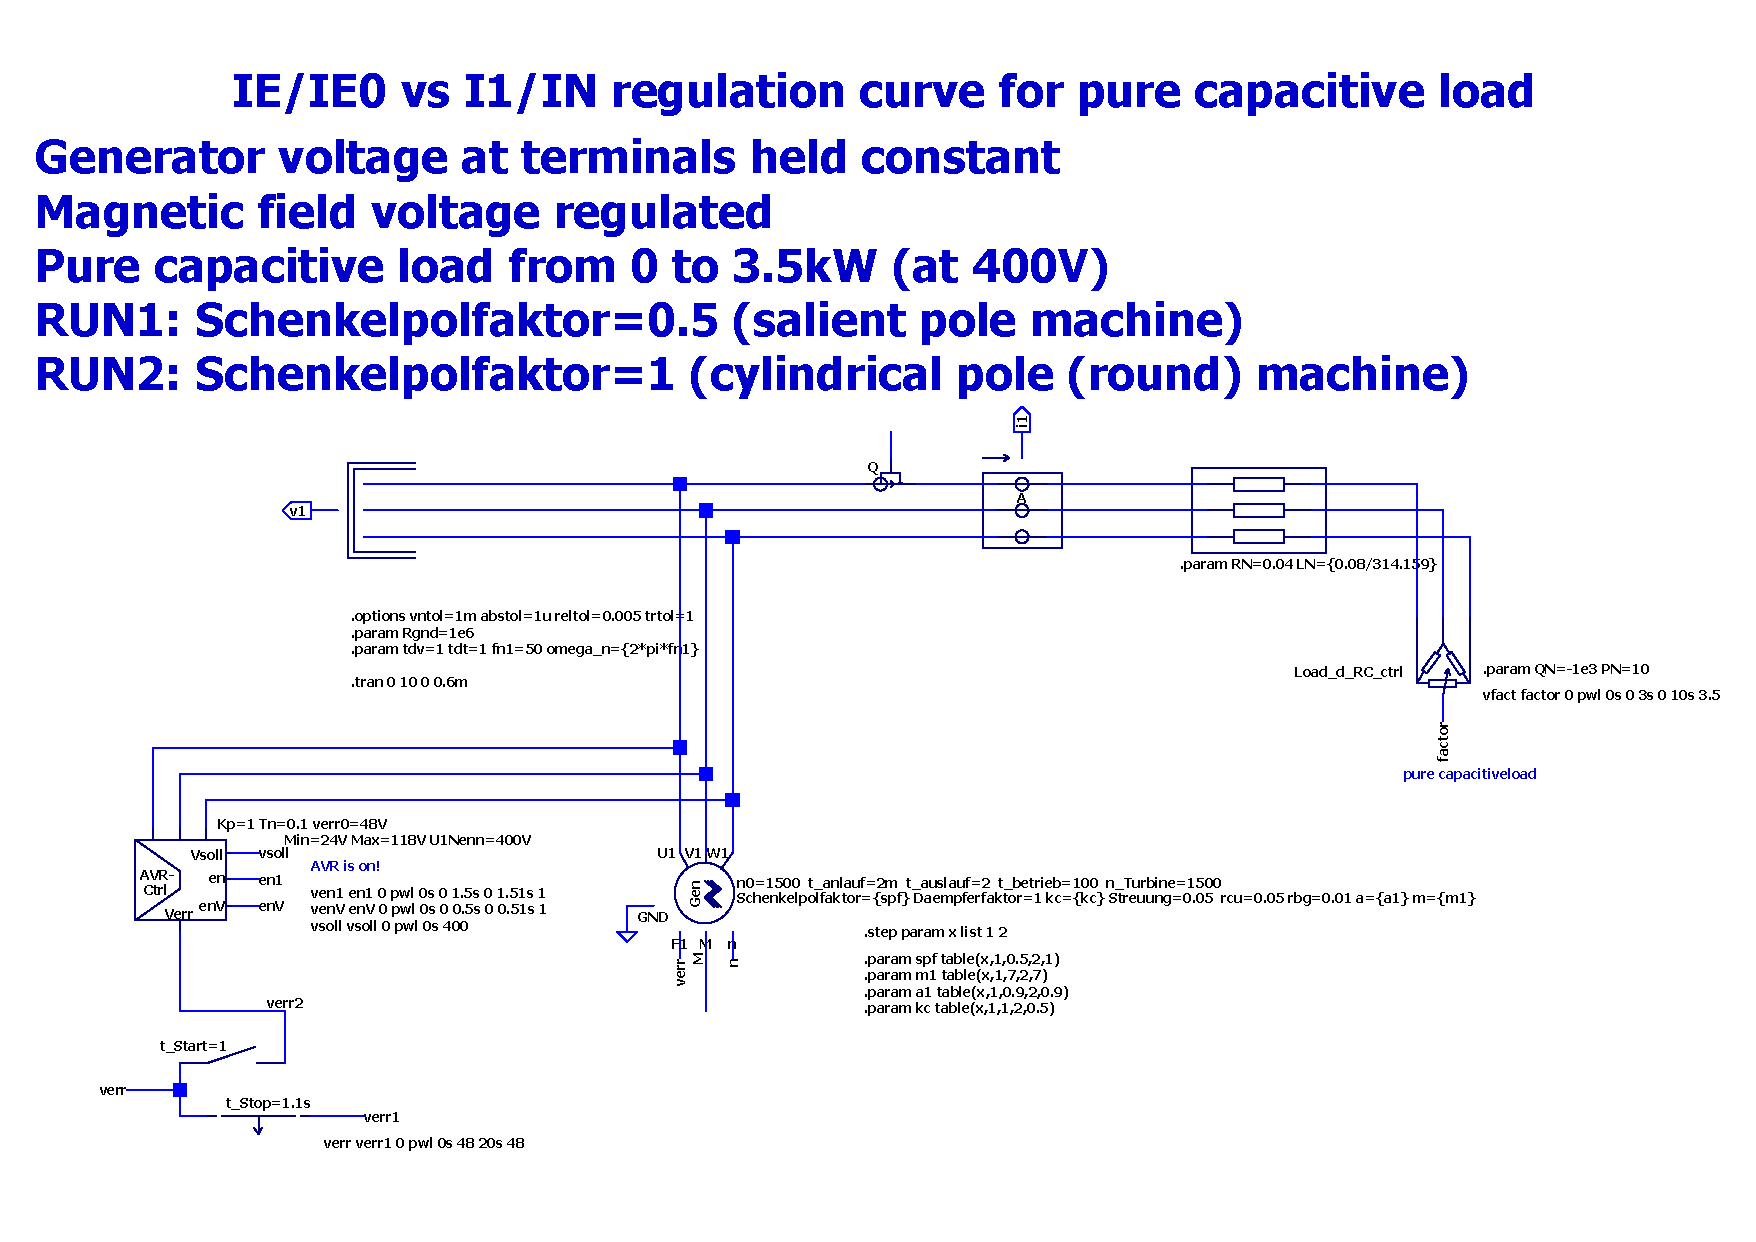
\includegraphics[width=0.9\textwidth] {figures/09_Synchronous_Generator_Characteristic_Curves_400V/sgen_400V_Regulationcurve_capacitive_schematic.pdf}
	\caption{Capacitive  Regulation curve - Schematic}
	\label{fig:figure915}
\end{figure}

\begin{figure}[H]
	\centering
	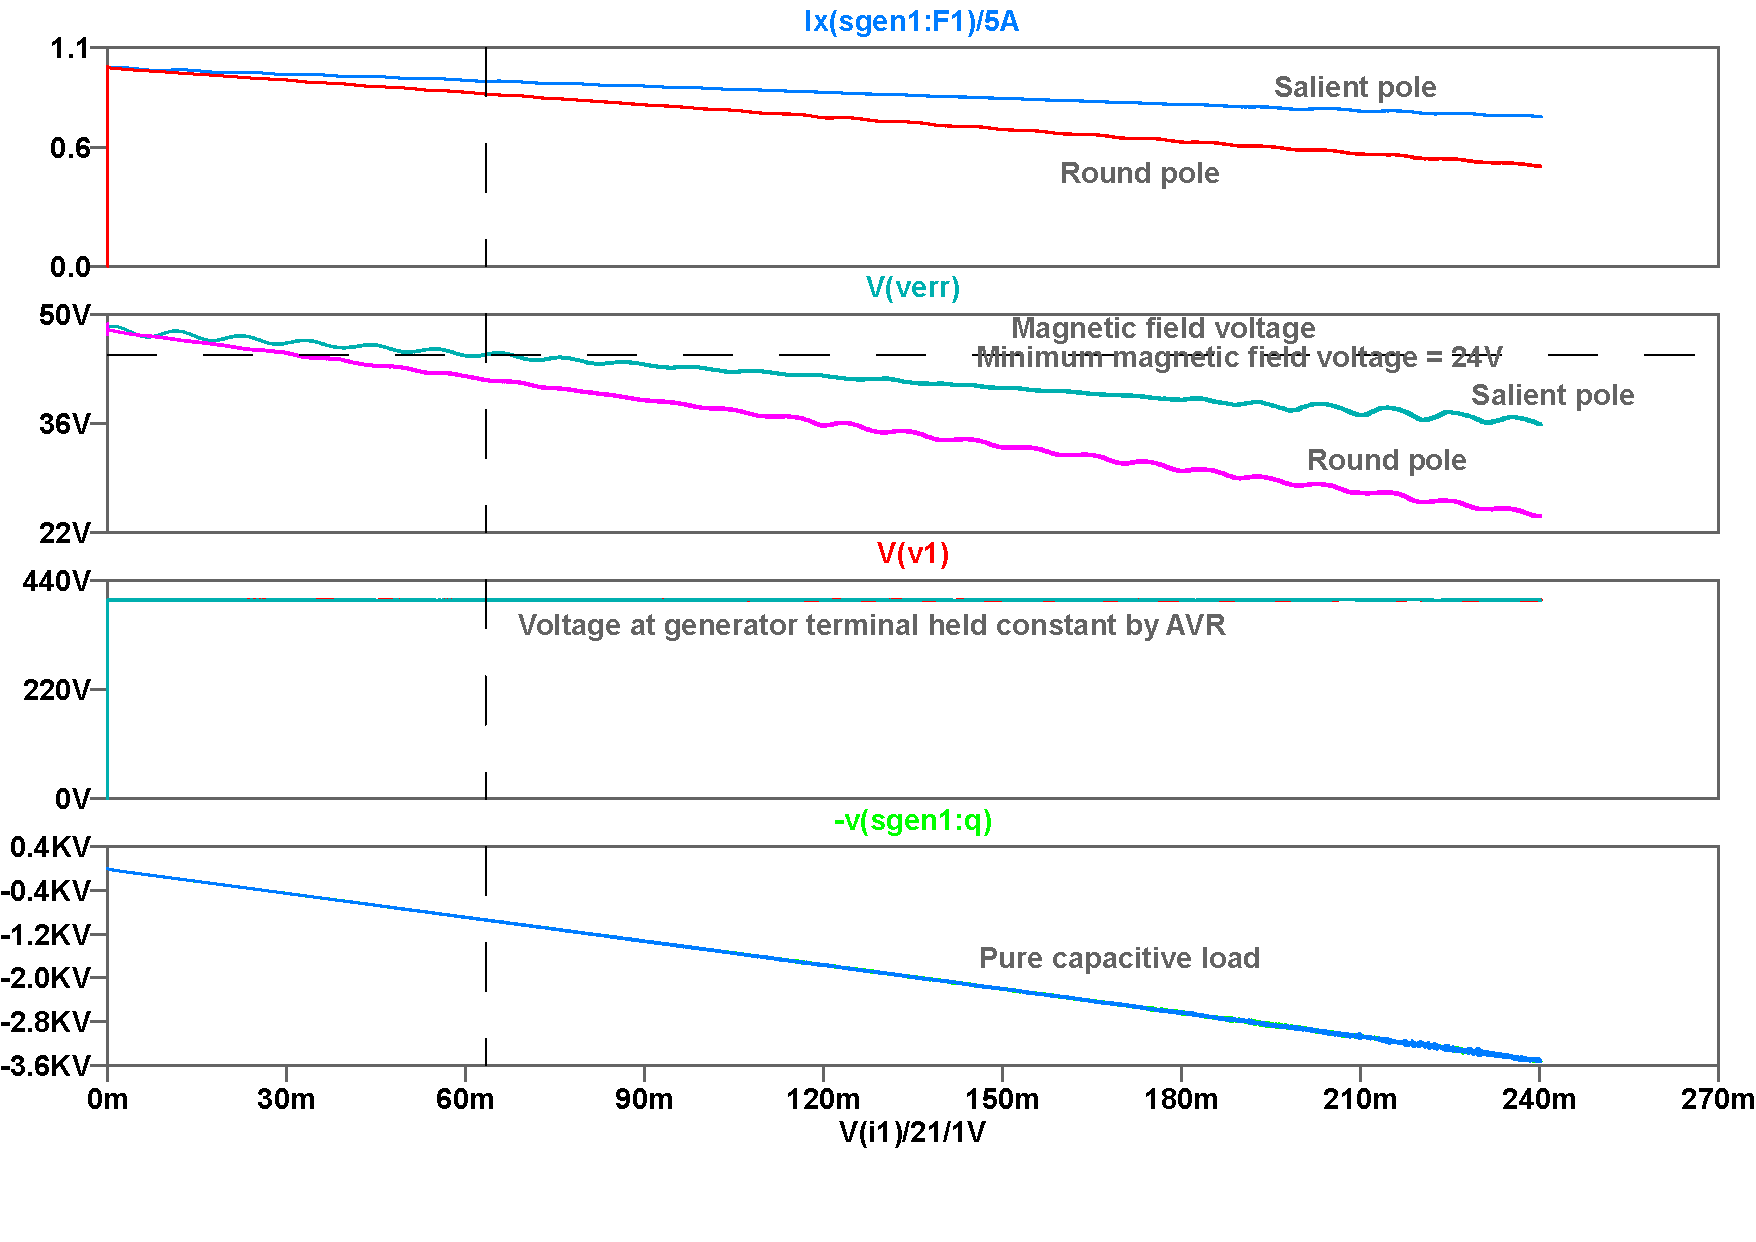
\includegraphics[width=0.9\textwidth] {figures/09_Synchronous_Generator_Characteristic_Curves_400V/sgen_400V_Regulationcurve_capacitive_waveform.pdf}
	\caption{Capacitive  Regulation curve - Waveform}
	\label{fig:figure916}
\end{figure}


% ============================================================
\section{V-Curves} see figure \ref{fig:figure917} and figure \ref{fig:figure918}  (simulation-file: same name as the heading) 
\label{sec:sg-v-curves}
% ============================================================

The V-curves of a synchronous machine show the relationship between stator
current and field current at constant active power and terminal voltage:

\begin{equation}
  I_s=f(I_f),
  \qquad
  P=\text{constant},
  \qquad
  U=\text{constant},
  \qquad
  f=\text{constant}.
  \label{eq:sg-v-curve-definition}
\end{equation}

The curves are named after their characteristic V-shaped appearance.

\subsection{Test Procedure}

The generator is connected to a stiff grid, which maintains approximately
constant voltage and frequency. The mechanical torque is adjusted to establish
a specified active-power output. The field current is then varied while the
mechanical power remains constant. For each excitation value, the stator
current, power factor, and reactive power are recorded.

\subsection{Minimum Stator Current}

For a balanced three-phase generator,

\begin{align}
  S &= \sqrt{3}\,U_{\mathrm{LL}}I_s, \\
  P &= \sqrt{3}\,U_{\mathrm{LL}}I_s\cos\varphi.
\end{align}

At constant active power and terminal voltage,

\begin{equation}
  I_s
  =\frac{P}{\sqrt{3}\,U_{\mathrm{LL}}\cos\varphi}.
  \label{eq:sg-v-curve-current}
\end{equation}

The stator current reaches its minimum when

\begin{equation}
  \cos\varphi=1.
\end{equation}

At this operating point, $Q\approx0$, and the generator exchanges almost no
reactive power with the grid.

\subsection{Underexcited Generator}

If the field current is reduced below the value corresponding to the minimum
stator current, the generator becomes underexcited. Under the usual generator
sign convention, it absorbs reactive power from the grid.

The stator current increases because it contains both an active-current and a
reactive-current component:

\begin{equation}
  I_s=\sqrt{I_P^2+I_Q^2}.
\end{equation}

Although the active power remains constant, the increasing reactive-current
component increases the total stator current. Excessive underexcitation can be
limited by stator heating, end-region heating, reduced steady-state stability,
and the risk of losing synchronism.

\subsection{Overexcited Generator}

If the field current is increased above the value corresponding to unity power
factor, the generator becomes overexcited and normally supplies reactive power
to the grid. The stator current again rises because the magnitude of the
reactive-current component increases.

Excessive overexcitation is limited mainly by rotor field-winding heating,
stator-current heating, magnetic saturation, and the maximum capability of the
excitation system.

\begin{remark}{Reactive-power sign convention}{rem:sg-q-sign}
The statements ``supplies reactive power'' and ``absorbs reactive power'' use
the generator convention. Some simulation programs define positive power as
power entering a component. In that convention, the displayed sign of $Q$ is
reversed and must be checked against the model reference directions.
\end{remark}

\subsection{Families of V-Curves}

A separate V-curve can be recorded for every active-power level, for example,

\begin{equation}
  P=0,
  \quad 0.25P_N,
  \quad 0.5P_N,
  \quad 0.75P_N,
  \quad P_N.
\end{equation}

As active power increases, the minimum possible stator current also increases:

\begin{equation}
  I_{s,\min}
  =\frac{P}{\sqrt{3}\,U_{\mathrm{LL}}}.
\end{equation}

The position of the minimum can shift slightly because of magnetic saturation,
stator resistance, and the synchronous-reactance voltage drop.

\subsection{Inverted V-Curves}

An inverted V-curve represents power factor as a function of field current:

\begin{equation}
  \cos\varphi=f(I_f).
\end{equation}

Its maximum occurs near unity power factor. On one side lies underexcited
operation; on the other lies overexcited operation. Moving away from the
maximum in either direction reduces the magnitude of the power factor and
increases stator current for the same active power.

\subsection{Relationship to Power Control}

The V-curves illustrate the approximate separation of active- and
reactive-power control when a synchronous generator is connected to a stiff
grid:

\begin{itemize}
  \item mechanical torque primarily controls active power $P$,
  \item field excitation primarily controls reactive power $Q$,
  \item the grid frequency fixes the average rotor speed, and
  \item the grid voltage largely fixes the terminal voltage.
\end{itemize}

This separation is not exact because excitation changes also influence the
load angle, saturation, stator current, and machine losses.

\begin{figure}[H]
	\centering
	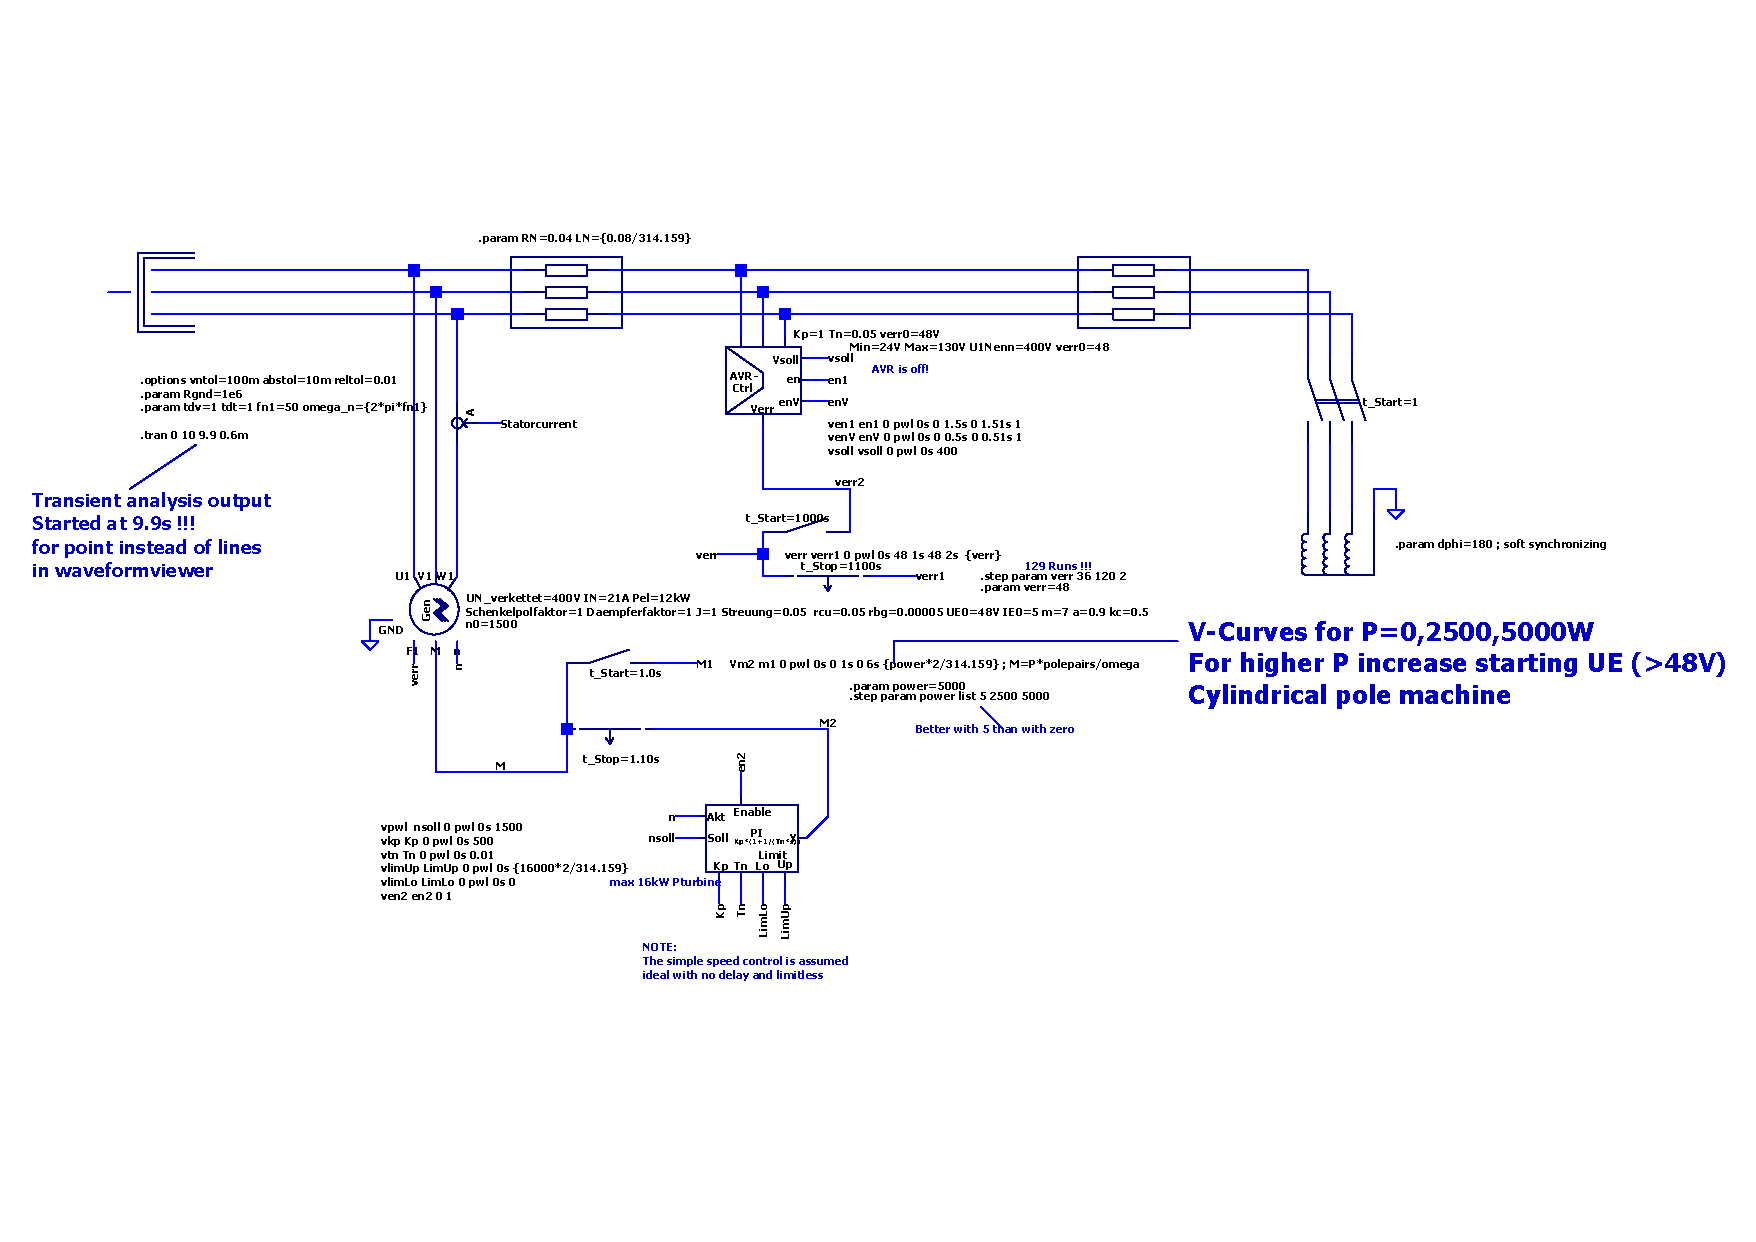
\includegraphics[width=0.9\textwidth] {figures/09_Synchronous_Generator_Characteristic_Curves_400V/sgen_400V_V_curves_multi_schematic.pdf}
	\caption{V-curve - Schematic}
	\label{fig:figure917}
\end{figure}

\begin{figure}[H]
	\centering
	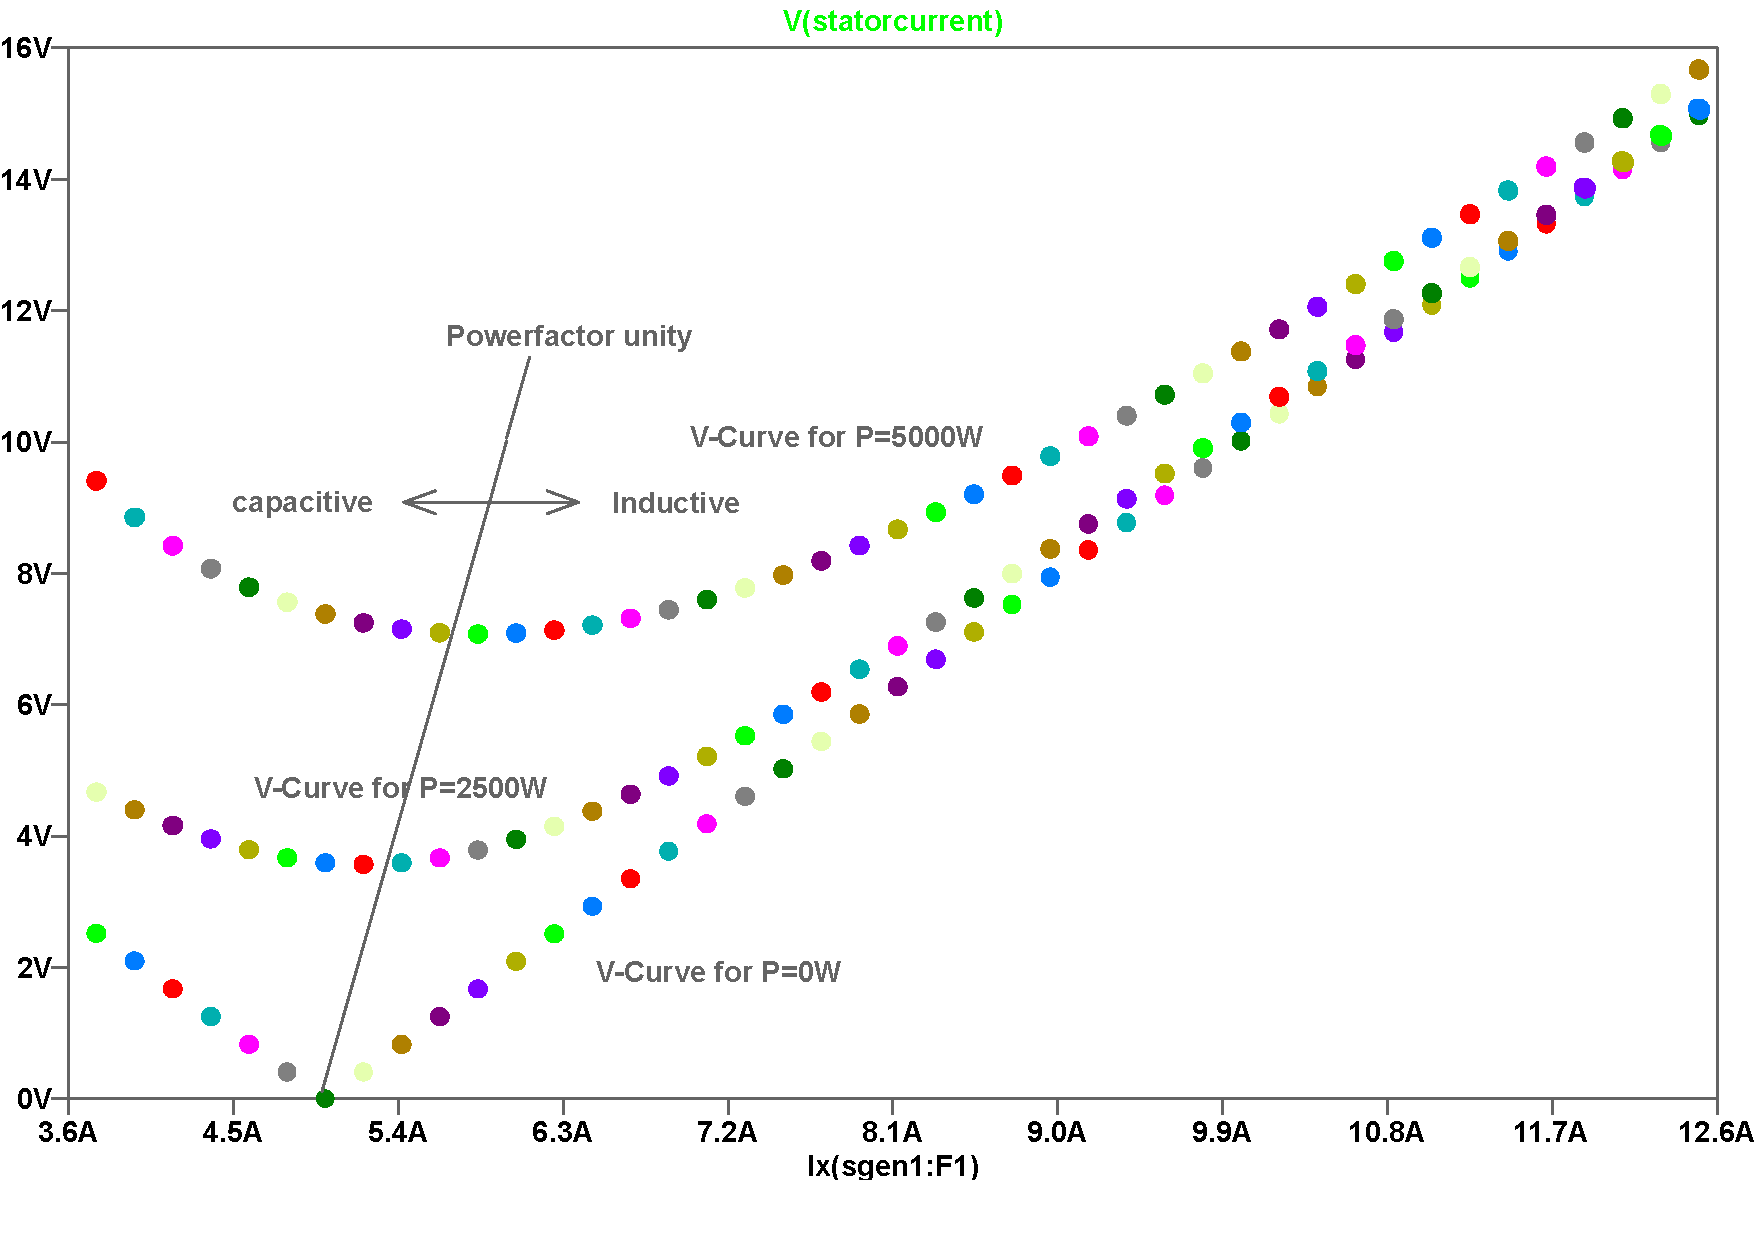
\includegraphics[width=0.9\textwidth] {figures/09_Synchronous_Generator_Characteristic_Curves_400V/sgen_400V_V_curves_multi_waveform.pdf}
	\caption{V-curve - Waveform}
	\label{fig:figure918}
\end{figure}

% ============================================================
\section{Comparison of the Characteristics}
\label{sec:sg-characteristic-comparison}
% ============================================================

\begin{table}[htbp]
  \centering
  \caption{Comparison of synchronous-generator characteristic curves}
  \label{tab:sg-characteristic-curves}
  \small
  \renewcommand{\arraystretch}{1.18}
  \begin{tabularx}{\textwidth}{@{}l c c Y Y@{}}
    \toprule
    \textbf{Characteristic} &
    \textbf{Horizontal axis} &
    \textbf{Vertical axis} &
    \textbf{Constant quantities} &
    \textbf{Main information} \\
    \midrule
    Open circuit & $I_f$ & $U_0$ & $I_s=0$, $n=n_N$ &
      Saturation and generated voltage \\
    Short circuit & $I_f$ & $I_k$ & $U=0$, $n=n_N$ &
      Steady-state fault current and synchronous impedance \\
    Load/external & $I_s$ & $U$ & $I_f$, $n$, $\cos\varphi$ &
      Natural terminal-voltage variation \\
    Regulation & $I_s$ & $I_f$ & $U$, $n$, $\cos\varphi$ &
      Excitation required for constant voltage \\
    V-curve & $I_f$ & $I_s$ & $P$, $U$, $f$ &
      Reactive-power and power-factor behaviour \\
    \bottomrule
  \end{tabularx}
\end{table}

The open-circuit and short-circuit characteristics are principally machine
test characteristics. Together, they provide information about saturation,
synchronous impedance, voltage regulation, and short-circuit ratio.

The load and regulation characteristics describe complementary operating
conditions. The load characteristic shows what happens when excitation remains
unchanged, whereas the regulation characteristic shows how excitation must be
adjusted to prevent the terminal voltage from changing.

The V-curves are mainly operating characteristics. They show the relationship
between excitation, stator current, power factor, and reactive power during
grid-connected operation.

\begin{chaptersummary}
The open-circuit characteristic describes generated voltage and magnetic
saturation. The short-circuit characteristic describes the steady-state fault
current and, together with the OCC, permits an approximate determination of
synchronous impedance and short-circuit ratio.

The load characteristic gives the terminal-voltage variation at constant
excitation, whereas the regulation characteristic gives the field current
required to keep voltage constant. V-curves show how underexcitation and
overexcitation increase stator current and determine whether a grid-connected
generator absorbs or supplies reactive power.
\end{chaptersummary}
